%%%%%%%%%%%%%%%%%%%%%%%%%%%%%%%%%%%%%%%%%%%%%%%%%%%%%%%%%%%%%%%%%%%%%%%%%%%%
% AGUJournalTemplate.tex: this template file is for articles formatted with LaTeX
%
% This file includes commands and instructions
% given in the order necessary to produce a final output that will
% satisfy AGU requirements, including customized APA reference formatting.
%
% You may copy this file and give it your
% article name, and enter your text.
%
%
% Step 1: Set the \documentclass
%
%

%% To submit your paper:
\documentclass[draft]{agujournal2019}
\usepackage{url} %this package should fix any errors with URLs in refs.
\usepackage{lineno}
\usepackage[inline]{trackchanges} %for better track changes. finalnew option will compile document with changes incorporated.
\usepackage{soul}
\linenumbers
%%%%%%%
% As of 2018 we recommend use of the TrackChanges package to mark revisions.
% The trackchanges package adds five new LaTeX commands:
%
%  \note[editor]{The note}
%  \annote[editor]{Text to annotate}{The note}
%  \add[editor]{Text to add}
%  \remove[editor]{Text to remove}
%  \change[editor]{Text to remove}{Text to add}
%
% complete documentation is here: http://trackchanges.sourceforge.net/
%%%%%%%

\draftfalse

%% Enter journal name below.
%% Choose from this list of Journals:
%
% JGR: Atmospheres
% JGR: Biogeosciences
% JGR: Earth Surface
% JGR: Oceans
% JGR: Planets
% JGR: Solid Earth
% JGR: Space Physics
% Global Biogeochemical Cycles
% Geophysical Research Letters
% Paleoceanography and Paleoclimatology
% Radio Science
% Reviews of Geophysics
% Tectonics
% Space Weather
% Water Resources Research
% Geochemistry, Geophysics, Geosystems
% Journal of Advances in Modeling Earth Systems (JAMES)
% Earth's Future
% Earth and Space Science
% Geohealth
%
% ie, \journalname{Water Resources Research}

\journalname{Enter journal name here}

%%%%% PERSONNAL MACROS and ENVIRONMENTS %%%%%%

\usepackage{bm} %bold symbols and letters in math mode, that stays italicized
%\usepackage{dutchcal} % \mathcal: also small letters. \mathbcal = bold ones. 
\DeclareFontFamily{OT1}{pzc}{}
\DeclareFontShape{OT1}{pzc}{m}{it}{<-> s * [1.10] pzcmi7t}{}
\DeclareMathAlphabet{\mathpzc}{OT1}{pzc}{m}{it}

\usepackage{amsmath}
\usepackage{amsfonts}
\usepackage{colortbl}

\usepackage{subfiles}
\usepackage{graphicx}
\graphicspath{{images/}} %for subfile graphics

\usepackage{siunitx} %SI units !
\sisetup{detect-all}
% \usepackage{biblatex}

\usepackage{caption}
%\usepackage{subcaption} %for subfigures 

%Delimiters
\newcommand\restrict[1]{\raisebox{-.5ex}{$|$}_{#1}} %restriction to a value 
\newcommand{\an}[1]{\ensuremath{\left\langle#1\right\rangle}} %angles
\newcommand{\sbra}[1]{\ensuremath{\left[#1\right]}} %square brackets []
\newcommand{\pbra}[1]{\ensuremath{\left\{#1\right\}}} %Poisson bracket {}
\newcommand{\parenthese}[1]{\ensuremath{\left(#1\right)}} %parentheses
\newcommand{\abs}[1]{\ensuremath{\left |#1\right |}} %absolute value
\newcommand{\norm}[1]{\left\lVert #1 \right\rVert} %norm

%Math Symbols
\newcommand{\g}{\mathbf{g}}
\newcommand{\dd}{\mathrm{d}}
\newcommand{\uu}{\tilde{u}}
\newcommand{\ww}{\tilde{w}}
\newcommand{\pp}{\tilde{p}}
\newcommand{\Ak}{\hat{A}_k}
\newcommand{\HH}{\mathcal{H}}
\newcommand{\ee}{{\rm e}}
\newcommand{\ii}{{\rm i}}
\newcommand{\Ks}{K_{\overline{\Sigma}}}
\newcommand{\R}{\mathbb{R}}
\newcommand{\ga}{\mathbf{\gamma}}
\newcommand{\al}{\mathbf{\alpha}}
\newcommand{\bb}{\mathbf{\beta}}
\newcommand{\K}{\mathbb{K}}


%Colored text
\definecolor{BlueGreen}{cmyk}{0.85,0,0.33,0}
\newcommand{\blu}[1]{{\color{BlueGreen} #1}}
\newcommand{\rose}[1]{{\color{magenta} #1}}    
\definecolor{mycolor}{RGB}{252,186,3}
\newcommand{\oran}[1]{{\color{mycolor} #1}}

%\usepackage{refcheck}
%%%
\definecolor{DodgerBlue}{RGB}{30,144,255}
\definecolor{peru}{RGB}{205,133,63}
%%%
\newcommand{\FLcom}[1]{\textcolor{DodgerBlue}{~\textit{(\textbf{FL:}~{#1})}}}
\newcommand{\FLadd}[1]{\textcolor{peru}{{#1}}}              
\newcommand{\FLdel}[1]{\textcolor{peru}{\sout{{#1}}}}     
\newcommand{\peru}[1]{\textcolor{peru}{{#1}}}              

%%%%%%%%%%%%%%%%%%%%%%%%%%%%%%%%%%%%%%%%%%%%%%%%%%%%%%%%%%%%%%
%%%%%%%%%%%%%%%%%%%%%%%%%%%%%%%%%%%%%%%%%%%%%%%%%%%%%%%%%%%%%%




\begin{document}

%% ------------------------------------------------------------------------ %%
%  Title
%
% (A title should be specific, informative, and brief. Use
% abbreviations only if they are defined in the abstract. Titles that
% start with general keywords then specific terms are optimized in
% searches)
%
%% ------------------------------------------------------------------------ %%

% Example: \title{This is a test title}

\title{Prior constraints and Bayesian estimation for an oceanic parameterization}

%% ------------------------------------------------------------------------ %%
%
%  AUTHORS AND AFFILIATIONS
%
%% ------------------------------------------------------------------------ %%

% Authors are individuals who have significantly contributed to the
% research and preparation of the article. Group authors are allowed, if
% each author in the group is separately identified in an appendix.)

% List authors by first name or initial followed by last name and
% separated by commas. Use \affil{} to number affiliations, and
% \thanks{} for author notes.
% Additional author notes should be indicated with \thanks{} (for
% example, for current addresses).

% Example: \authors{A. B. Author\affil{1}\thanks{Current address, Antartica}, B. C. Author\affil{2,3}, and D. E.
% Author\affil{3,4}\thanks{Also funded by Monsanto.}}

\authors{=list all authors here=}


% \affiliation{1}{First Affiliation}
% \affiliation{2}{Second Affiliation}
% \affiliation{3}{Third Affiliation}
% \affiliation{4}{Fourth Affiliation}

\affiliation{=number=}{=Affiliation Address=}
%(repeat as many times as is necessary)

%% Corresponding Author:
% Corresponding author mailing address and e-mail address:

% (include name and email addresses of the corresponding author.  More
% than one corresponding author is allowed in this LaTeX file and for
% publication; but only one corresponding author is allowed in our
% editorial system.)

% Example: \correspondingauthor{First and Last Name}{email@address.edu}

\correspondingauthor{=name=}{=email address=}

%% Keypoints, final entry on title page.

%  List up to three key points (at least one is required)
%  Key Points summarize the main points and conclusions of the article
%  Each must be 140 characters or fewer with no special characters or punctuation and must be complete sentences

% Example:
% \begin{keypoints}
% \item	List up to three key points (at least one is required)
% \item	Key Points summarize the main points and conclusions of the article
% \item	Each must be 140 characters or fewer with no special characters or punctuation and must be complete sentences
% \end{keypoints}

\begin{keypoints}
    \item \blu{à revoir !}
    \item Sobol' global sensitivity analysis, a rigorous method relying on variance decomposition, is used to identify the most influential parameters of the EDMF parameterization. 
    \item Entrainment coefficient and plume fractional area at the surface are the most influential parameters, since they control the activation of the mass-flux scheme
    \item Bayesian inference, via a simple MCMC algorithm, is used to estimate the full posterior density of the parameters, conditioned on LES data.
    \item With only two LES experiments, MCMC is found to be computationally expensive, motivating the use of emulators or global approximations of the posterior.
\end{keypoints}

%% ------------------------------------------------------------------------ %%
%
%  ABSTRACT and PLAIN LANGUAGE SUMMARY
%
% A good Abstract will begin with a short description of the problem
% being addressed, briefly describe the new data or analyses, then
% briefly states the main conclusion(s) and how they are supported and
% uncertainties.

% The Plain Language Summary should be written for a broad audience,
% including journalists and the science-interested public, that will not have 
% a background in your field.
%
% A Plain Language Summary is required in GRL, JGR: Planets, JGR: Biogeosciences,
% JGR: Oceans, G-Cubed, Reviews of Geophysics, and JAMES.
% see http://sharingscience.agu.org/creating-plain-language-summary/)
%
%% ------------------------------------------------------------------------ %%

%% \begin{abstract} starts the second page

\begin{abstract}
[ enter your Abstract here ]
\end{abstract}

\section*{Plain Language Summary}
[ enter your Plain Language Summary here or delete this section]


%% ------------------------------------------------------------------------ %%
%
%  TEXT
%
%% ------------------------------------------------------------------------ %%

\section{Introduction}
%
% \begin{enumerate}
%     \item Uncertainty 
%     \item direct and reverse propagation
%     \item In AOGCM, uncertainty comes from: 1 knowledge of initial and boundary conditions (Charney, Lorenz) --> data assimilation, 2 errors representation of physical processes / params, 3 adequate free parameters, 4 adequacy of resolved dynamics (hydro/NH), and most errors in particular its discretization and properties (spurious mixing in ocean) <-- tout ça c'est peut-être dans intro générale en fait...
%     \item 2 and 3 goes together, since 3 can inform the devt of 2
%     \item State of the art: reverse tuning of GCM
%     \item Hourdin: passer aux process pour éciter compensation d'erreurs
%     \item Process, with different approaches: Hourdin, Souza, Wagner, Dunbar (Kalman, relire?) 
%     \item direct: short reviews of methods (citer Qiao reviews paper)
%     \item Sobol' analysis (citer books et review papers)
%     \item examples in ESM: 
%     % \begin{itemize}
%     %     \item https://agupubs.onlinelibrary.wiley.com/doi/pdfdirect/10.1002/2017JD027348
%     %     \item https://www.jstor.org/stable/pdf/48639049.pdf?casa_token=tSpbphoLhNcAAAAA:eVwy8K0iR4nJaWqBvBL79sDJAKx58EDfeB2LIzESjACBLeBLJDGJMjm_oqZNPBuZbNDdAs4IAqUQxd4uM87p5WjzoY0-i3m4He3exELebuZnzttQew
%     %     \item hydro : file:///home/manolis/Downloads/water-07-02924-v2.pdf
%     % \end{itemize} 
%     \item examples for params: Pelletier.
% \end{enumerate}
% \blu{faire intro sur quantif incertitude}.
% \blu{écrire une intro avec  un vrai plan qui explique l'articulationn entre sens anal, estimation est plus géénralement quantif inertitudes. Dire que avant de comparer aux obs pour calibre, il faut savoir quels paramètres sont importants.}
% \blu{Intro thèse Qiao: factor prioritisation: put most effort in calibrate very influential parameters different from factor fixing: fix non ionfluential parameters to nominal values}
% \\
% \blu{Couvreux 2021 tuning "However, it is often con-
% ducted without much control on the way it modifies the parameterization behavior at the process level as
% the calibration focuses more on regional or global constraints, such as the radiative balance of the Earth
% System for climate models, or performance metrics"}
% \\
% \blu{Souza:  Uncertain parameters are then adjusted to minimize the loss function. One
% can also estimate the standard deviation around the optimal values by computing the Hessian of the loss
% function (Sraj et al., 2014; Thacker, 1989).
% \\
% the power of Bayes' formula is that it can reveal distinct parameter regimes, the
% existence of multiple maxima, relationships between parameters, and the likelihood of parameter values
% relative to optimal ones.
% }
% \\
% \blu{faire le cas de WANG1 ??}

% \blu{IMPORTANT QUESTION FOR OLIVIER: comment concilier que dans Sobol' on suppose paramètres indépendants, et dans calibration on trouve que ya des corrélations (mais avec conditionnement aux obs) }
%%%%
%
% \blu{KPP with NN }
% https://agupubs.onlinelibrary.wiley.com/doi/full/10.1029/2024MS004405
%
%

In numerical models of ocean and atmosphere, errors  (or uncertainties) can originate from several sources: \textit{(i)} incomplete knowledge of initial or boundary conditions, a challenge recognized since the early days of modeling \cite{charney_dynamic_1951,lorenz_deterministic_1963}, which has driven significant advancements in data assimilation; \textit{(ii)} the accuracy of resolved (thermo-)dynamical equations and their discretization, potentially introducing structural errors \cite{lauritzen_reconciling_2022,fox-kemper_challenges_2019,mesinger_numerical_2018,klingbeil_numerics_2018}; \textit{(iii)} the ability of physical parameterizations to represent effects of subgrid processes on resolved scales; \textit{(iv)} incomplete knowledge of the parameters involved in these parameterizations; and \textit{(v)} the coupling of parameterizations and dynamical cores \cite{gross_physics_2018}. In this chapter, we will focus on uncertainty quantification (UQ) of the "free" parameters in parameterizations, and how UQ can inform their development. Conversely, we will also demonstrate how physical and mathematical constraints can inform UQ efforts. 
%%%%
\par Uncertainty quantification aims at characterizing and quantifying the uncertainty of a model output $F(\bm X)$ and its input parameters $\bm X$. UQ can be divided into two classes of problems: forward and inverse propagation of uncertainty. Forward problems, encompassing sensitivity analysis, consist in evaluating how uncertainty in the parameters will affect outputs of the model and produce output variability. Forward problems do not require the use of observational data. The aim of inverse problems is to identify model biases and/or estimate the values or distribution of parameters, based on a comparison of outputs to observations. 
%
\par This estimation (a.k.a. calibration or "tuning") of the model parameters is an unavoidable task to perform before any practical or operational usage of a model. For oceanic regional models, Numerical Weather Prediction (NWP) models, as well as atmospheric and oceanic Global Circulation Models (GCMs) constituting Earth System Models (ESMs), calibration has usually been performed manually at the level of the full model. Parameters are then used as degrees of freedom to match global metrics assessing the realism of the models, such as radiative balance for atmospheric GCMs \cite{hourdin_art_2017}. However, this strategy does not ensure that each parameterization still correctly predicts local physical processes and thus is prone to allow error compensation between parameterizations, hiding structural biases of the models. In order to overcome this pitfall, \citeA{hourdin_art_2017} propose the following hierarchical procedure: a first tuning of each parameterization at the level of local physical processes, then an independent tuning of each model constituting an ESM, and eventually a tuning of the fully coupled ESM. In order to avoid user-based biases in the calibration, there is a growing interest in automatic statistical estimation methods, with or without the usage of surrogate models, at each of these steps \cite{hourdin_art_2017,schneider_earth_2017}. These methods also possess the advantage to estimate parameter distributions or ranges of acceptable values that can be reused for the next calibration step. 
%
\par In this chapter, we focus on the small scale physical process level. The usage of several statistical estimation approaches for parameterizations can be found in the literature, taking advantage of a systematic comparison of 1D parameterizations output with averaged Large-Eddy Simulation (LES). Bayesian estimation is designed to estimate the full probability distribution of the parameters. While estimation can be performed using a "brute force" exploration of the parameter space via Monte-Carlo-Markov-Chain (MCMC) algorithms \cite{souza_uncertainty_2020}, more refined methods such as Ensemble or Unscented Kalman Inversion \cite{dunbar_calibration_2021,wagner_formulation_,lopez-gomez_training_2022} have shown improved efficiency at the expense of a Gaussian approximation of the parameters' distribution. 
Alternatively, history-matching --accelerated by Gaussian-processes emulators of the parameterization \cite{couvreux_processbased_2021}--, is designed to identify, in a Manichean way, acceptable and non-acceptable ranges of parameters. In opposition to classical Bayesian inference, this method purposely do not provide further nuance in order to avoid overfitting to the training dataset. All these methods rely on the choice of appropriate metrics (or loss functions) and estimation of model and observational errors. 
%
%
\par Although calibration has a prominent role to achieve realistic simulations, forward uncertainty quantification of the outputs to uncertainty in the input parameters can be an interesting tool to understand model behaviors. It is performed sometimes during the development stage of a parameterization, for few parameters expected to be the most sensitive based on developer's knowledge. Sensitivity analysis is usually performed manually by changing the value of the parameter of interest, while keeping the other constants  -- a technique referred as \textit{one-at-a-time screening} by statisticians \cite<e.g.>{morris_factorial_1991,murphy_quantification_2004}. Since other parameters are kept constant, this method is a \textit{local} sensitivity analysis. It can potentially miss other sensitive parts of the parameter space or significant interactions in parameter variations. \textit{Global} sensitivity analysis methods aim at remedying these issues by performing a systematic exploration of the whole parameter space \cite{iooss_review_2015,gan_sensitivity_2018}% \blu{parcourir et citer si pertinent https://gmd.copernicus.org/articles/16/1395/2023/gmd-16-1395-2023.html}
Sobol' variance decomposition \cite{sobol_sensitivity_1993} is one of the method providing the most complete information on parameter's sensitivity and their higher order interactions. However, it requires numerous model evaluations that can be prohibitive for complex models, obviating the need for emulators. Applications of Sobol' analysis can be found in the ocean/atmosphere literature for the study of simplified climate models \cite{cao_global_2020a} and 3D NWP models \cite<with the help of Gaussian process emulator,>{ji_assessing_2018,baki_determining_2022}. At the level of physical processes, it has been used by \citeA{pelletier_sensitivity_2018} to build accurate metamodels of air-sea interactions bulk formula with reduced complexity.
%  The accuracy of the method comes at the expense of a large number of model evaluations (1000$\times$ the number of parameters), which are however affordable for single-process parameterizations models ($O(\SI{1}{h})$ for $O(10^5)$ evaluations of the EDMF parameterization on a 8 core laptop).
%%%
%
\par Being either for inverse or forward UQ, it should be noted that the methods cited above and their applications to ocean and atmosphere are gradient-free: they do not require the knowledge of the gradient or adjoint of the model. However, gradient-based UQ methods are generally more efficient, motivating the development of automatic differentiation tools for models written in \texttt{Fortran} \, or the rewriting of codes in more natively differentiable languages, such as \texttt{Julia} \cite{ramadhan_oceananigansjl_2020} or \texttt{Jax} \cite{hafner_veros_2018}. 
%%%
\par In this chapter, we recall in section \ref{sec: model description} the EDMF model formulation, identify input parameters and output variables of interest. In section \ref{sec: prior}, we derive prior constraints on parameters' range based on physical and mathematical constraints. In section \ref{sec: sobol} we perform a global sensitivity analysis of the model using Sobol' method, and identify the most and least influential parameters. In section \ref{sec: inverse}, we present the Bayesian approach to solve inverse UQ problems, and apply it to the EDMF model. 
%
%
\section{Model description}\label{sec: model description}
%
We start with the SCM (i.e. 1D) equations for mean temperature, salinity and horizontal velocity, 
%
\begin{eqnarray*}
    \begin{cases}
        \partial_t \overline{\theta} = \frac{\overline{\epsilon}_\nu }{c_p - \alpha gz } - \partial_z \overline{w' \theta'} \label{eq:temp budget}
        \\
        \partial_t \overline{S} = - \partial_z \overline{w' S'}
        \\
        \partial_t \overline{\bm u}_h = - \partial_z \overline{w' \bm u_h'} 
    \end{cases}
\end{eqnarray*}
%
where turbulent fluxes of the form $\overline{w'X'}$ (with $X=\theta,S,\bm u_h$) are closed according to the Eddy-Diffusivity Mass-Flux (EDMF) parameterization:
%
\begin{eqnarray*}
    \overline{w'X'} = \underbrace{-K_X \partial_z \overline{X}}_{\rm{ED}} + \underbrace{a_p w_p (X_p - \overline{X})}_{\rm{MF}}
\end{eqnarray*}
%
Eddy viscosity $K_u$ and diffusivities $K_\theta=K_S$ 
in turbulent vertical fluxes are computed from a turbulence closure model based on a 
prognostic equation for the turbulent kinetic energy (TKE) and a diagnostic 
computation of appropriate length scales (a.k.a. 1.5-order turbulence closure; see chapter \ref{chap: EDMF2}). The mass-flux contributions are computed via the plume model
%
\begin{eqnarray}\label{eq: plume model}
    \begin{cases}
        \partial_z (a_p w_p) = E-D
        \\
        a_p w_p \partial_z \theta_p = E (\overline{\theta} - \theta_p)
        \\
        a_p w_p \partial_z S_p = E (\overline{S} - S_p)   
        \\
        a_p w_p \partial_z \bm u_{h,p} = E (\overline{\bm u}_h - \bm u_{h,p}) + a_p w_p \peru{C_u} \partial_z   \overline{\bm u}_h 
        \\
        a_p w_p \partial_z w_p = - \peru{b} E w_p + \peru{a} a_p (b_{\rm{eos}}(\theta_p, S_p) - b_{\rm{eos}}(\overline{\theta},\overline{S}) ) +\peru{ b'} \frac{1}{h} a_p (w_p)^2 
        \\
        E = a_p \peru{C_{\rm ent}} \max (0,\partial_z w_p)
        \\
        D = -a_p \peru{C_{\rm det}} \min (0,\partial_z w_p) - a_p w_p \peru{\delta_0}\frac{1}{h}
    \end{cases}
\end{eqnarray}
%
along with boundary conditions at the ocean surface $z=0$:
%
\begin{eqnarray*}
    && \theta_p (z=0) = \overline{\theta}(z=0), \qquad S_p (z=0) = \overline{S}(z=0), \qquad \bm u_{h,p} (z=0) = \overline{\bm u_h}(z=0), 
    \\
    && w_p (z=0) = \peru{w_p^0}, \qquad a_p(z=0) = \peru{a_p^0}
\end{eqnarray*}
%
Along with surface boundary conditions for plume area and vertical velocity $\peru{a_p^0}$ and $\peru{w_p^0}$, orange parameters in plume equations  
 forms the \textit{input} parameters that we want to calibrate: $\bm X = (\peru{C_{\rm ent}}, \peru{C_{\rm det}}, \peru{C_u}, \peru{a}, \peru{b}, \peru{b'}, \peru{\delta_0}, \peru{a_p^0}, \peru{w_p^0})$. Note that the TKE equation also contains adjustable parameters. However, we do not include them in the estimation procedure, since we aim to recover the standard TKE scheme in non-convective conditions \cite<for an automatic calibration of an atmospheric TKE scheme, we refer to>{vignon_designing_2024}. Let us write $\mathcal{D}=[-H,0]\times[0,T]$ the spatio-temporal domain of the simulation. Then the following outputs of the model $Y =  \pbra{\overline{\theta}(z,t) }_{(z,t)\in \mathcal{D}}, \pbra{\overline{S}(z,t)}_{(z,t)\in \mathcal{D}} , \pbra{\overline{\bm u}_h(z,t)}_{(z,t)\in \mathcal{D}}$ are chosen as \textit{variables of interest} for uncertainty quantification and would be treated independently. This choice is motivated by the fact that mean fields are the ultimate target of the 3D models that would contain EDMF parameterization. We do not use quantities internal to the parameterization (such as plume variables) since reference profiles derived from Large Eddy Simulation (LES) can be sensitive to the method of e.g. plume identification \cite{couvreux_processbased_2021}.
 The UQ problem can thus be recast in the form
 %
 \begin{eqnarray}\label{eq: model}
    Y = F(\bm X ; \bm C_{\rm exp} )
 \end{eqnarray}
%
where $F$ is the model and $\bm C_{\rm exp}$ is a hyperparameter containing all the information of idealized experiments such as initial and boundary conditions. 
%
\section{Prior constraints on parameters}\label{sec: prior}
%
Prior knowledge  on parameters can be derived from either physical or numerical constraints.
%
\paragraph{$C_{\rm ent}$ and $C_{\rm det}$:}
%
Constraints on $C_{\rm ent}$ and $C_{\rm det}$ can be derived from the physical constraint $0\leq a_p \leq 1$. A sufficient condition to ensure that $a_p \leq 1$ at any depth is to impose $\partial_z a_p \geq 0$, which is consistent with profiles obtained from conditional sampling (chapter \ref{chap: EDMF2}). The equation for $a_p$ can be combined with entrainment/detrainment closures to give
%
\begin{eqnarray*}
    \partial_z a_p = a_p \frac{\delta_0}{h} + 
    \begin{cases}
        (1-C_{\rm ent}) a_p \frac{\partial_z w_p}{-w_p} \text{ if } \partial_z w_p \geq 0
        \\
        (1-C_{\rm det}) a_p \frac{\partial_z w_p}{-w_p} \text{ if } \partial_z w_p < 0             
    \end{cases}
\end{eqnarray*}
%
Recalling that $w_p<0$, sufficient conditions to have $\partial_z a_p \geq0$ are $C_{\rm ent} \leq 1$, $C_{\rm det} \geq 1$ and $\delta_0 \geq 0$. Moreover, we show in appendix C3 of chapter \ref{chap: EDMF2} that $C_{\rm det} <2$ is a sufficient numerical condition to ensure that $a_p \geq 0$. As a summary, we have
%
\begin{eqnarray*}
    0 \leq C_{\rm ent} \leq 1, \qquad 1 \leq C_{\rm det} \leq 2
\end{eqnarray*}

\paragraph{$C_u$:}
%
In section 4.4 of chapter \ref{chap: EDMF1}, we derived the following vertically integrated resolved kinetic energy budgets
%
\begin{eqnarray*}
    \partial_t \an{ E_k }_z &=& - \an{  K_u (\partial_z \overline{\bm u}_h)^2  }_z - \an{ \frac{E + D}{2 (1-C_u) } (\bm u_{h,p} - \overline{\bm u}_h)^2 }_z 
\\
 &&  - \sbra{ \overline{\bm u}_h \cdot \overline{w'\bm u_h' } }_{- H}^0- \sbra{ \frac{a_p w_p}{2 (1- C_u)} (\bm u_{h,p} - \overline{\bm u}_h)^2  }_{- H}^0
\end{eqnarray*}
%
where $\an{ X }_z = 1/H\int_{- H}^0 X  \, \dd z$, and the boundary operator is
$\sbra{X}_{- H}^0 = 1/ H (X(z=0) - X(z=-H) )$.
Since the term $- \an{ \frac{E + D}{2 (1-C_u) } (\bm u_{h,p} - \overline{\bm u}_h)^2 }_z $ is associated to a transfer from mean kinetic energy to TKE due to entrainment and detrainment processes, it should remain negative. Thus, it implies that $C_u < 1$. Additionally, according to \citeA{wu_effects_1994} we must impose $C_u \geq 0$. As a summary, 
%
\begin{eqnarray*}
    0 \leq C_u < 1
\end{eqnarray*}
%
\paragraph{$a$ and $b$:}
%
The parameters $a$ and $b$ have been introduced respectively as a reduced virtual mass term \cite<e.g.>{bretherton_new_2004} -- representing the \textit{reduction} of plume
buoyancy due to pushing and pulling on the environment -- and a \textit{reduced} entrainment term. Thus, by definition we have 
%
\begin{eqnarray*}
    0 \leq a \leq 1, \quad  0 \leq b \leq 1
\end{eqnarray*}
% %
% \begin{table}
%     \includegraphics[width=\textwidth]{\figPATH de_roode_table.png}
%     \label{tab: de roode}
%     \caption{Overview of values used for the constants $a$ and $b$ in the parameterized vertical velocity for shallow cumulus clouds, from \citeA{roode_parameterization_2012}. $w_c$ indicates the in-cloud vertical velocity, corresponding to our plume velocity $w_p$.}   
% \end{table}
%
\paragraph{$b'$ and $\delta_0$:}
%
We were not able to find a clear constraint on these parameters. Values can be found around $0.3$ \cite{gregory_estimation_2001,tan_extended_2018,turner_buoyancy_1979}. Thus, we adopt the following range
%
\begin{eqnarray*}
    0 \leq b' \leq 3, \qquad 0 \leq \delta_0 \leq 3
\end{eqnarray*}
%
\paragraph{$a_p^0$ and $w_p^0$:}
%
The plume equations \eqref{eq: plume model} are derived assuming that $a_p \ll 1$. Thus, we restrict its surface value to 0.5 in order to avoid inconsistencies. Equation for the plume vertical velocity can lead to positive and negative solutions. In order to select negative solutions of the ODE, we adopted a minimal vertical velocity at the surface $w_p^0= \SI{-1e-8}{m.s^{-1}}$ in chapter \ref{chap: EDMF2}. Without no more knowledge, we propose to vary logarithmically this parameter over several decades, leading to
\begin{eqnarray*}
    0 \leq a_p^0 \leq 0.5, \qquad \SI{-1e-8}{m.s^{-1}} \leq w_p^0 \leq \SI{-1e-1}{m.s^{-1}}
\end{eqnarray*}
%
% \blu{REFAIRE TOUT avec CES VALEURS--> pb, c'est très sensible à la valeur de wp0!}
% \begin{eqnarray*}
%     0 \leq a_p^0 \leq 0.5, \qquad \SI{-1e-8}{m.s^{-1}} \leq w_p^0 \leq \SI{-1e-7}{m.s^{-1}}
% \end{eqnarray*}
%
%
\section{Sensitivity analysis}\label{sec: sobol}
%
The goal of sensitivity analysis is to quantify how changes in input parameters will affect outputs variables, regardless of observation data. In particular, it can help assess whether uncertainty on parameters will propagate on the variables of interest. To do so, we use Sobol' analysis \cite{sobol_sensitivity_1993}, which is a variance-based sensitivity analysis. This method is applicable only for independent parameters\footnote{For global sensitivity analysis on dependent inputs, recent studies suggest the use of Shapley values \cite{owen_sobol_2014,owen_shapley_2017}}.
In such framework, (uncertain) input parameters $\bm X$ are considered as random variables which in turn results in a random output $Y = F(\bm X)$. Uncertainty of the output is quantified by the variance of $Y$. Then \textit{first order} -- or \textit{main effect} -- Sobol' indices quantify what is the direct contribution of each parameter $X_i$ to this total variance. In practice one considers $\mathbb{E}\sbra{Y | X_i}$, the expectation of $Y = F(\bm X)$ conditioned on $X_i$. In $\mathbb{E}\sbra{Y | X_i}$ all the randomness due to other parameters $X_{j\neq i}$ is averaged. The remaining variability is directly due to $X_i$, and can be quantified by the normalized variance 
%
\begin{eqnarray}\label{eq: 1st sobol}
    S_i = \frac{\textrm{Var} \parenthese{\mathbb{E} \sbra{Y | X_i }}}{\textrm{Var}(Y)} = \frac{\mathbb{E} \sbra{\norm{ \mathbb{E} \sbra{Y | X_i} - \mathbb{E} \sbra{Y} }^2}} {\mathbb{E}  \sbra{\norm{ Y - \mathbb{E}\sbra{Y} }^2}}, \qquad 0 \leq S_i \leq 1
\end{eqnarray}
%
where $S_i$ is named first order Sobol' index and $\textrm{Var}$ denotes variance. 
%
A high value indicates that direct variations of $X_i$ influence significantly the output. However, a small value does not necessarily indicate that a parameter is unimportant. Indeed, its influence could arise from simultaneous variations with other parameters. The \textit{total Sobol' index} measures the interactions of $X_i$ with all other parameters, and can be computed as 
%
\begin{eqnarray*}
    S_i^{\rm tot} = 1 - \frac{\textrm{Var} \parenthese{\mathbb{E} \sbra{Y | \pbra{ X_j}_{j \neq i} }}}{\textrm{Var}(Y)}, \qquad   S_i^{\rm tot} \geq S_i
\end{eqnarray*}  
%
Consequently, a high first order index means that the parameter is important, while a low total index means that the parameter is unimportant.
% \blu{high first order index means that the parameter is important, low total index means that the parameter is not important}
% In practice such indices can be computed via the \textit{pick\&freeze} formula \blu{ref à chercher dans le papier de Qiao}. Let us fix the parameter of interest as $X_i = X_1$, denote $\bm Z = (X_2, \ldots X_d)$ the remaining parameters and let $X_1',\bm Z'$ be an independents copies of $X_1,\bm Z$, i.e. $X_1,\bm Z$ and $X_1',\bm Z'$ are uncorrelated but possess the same distribution. Denote also $Y' = F(X_1',\bm Z')$ and $\tilde{Y} = F(X_1, \bm Z')$. Then \citeA{sobol_sensitivity_1993} prooved that 
%
In practice such indices can be computed via the \textit{pick\&freeze} formula \cite{sobol_sensitivity_1993}. Let us fix the parameter of interest as $X_i = X_1$ and consider $\bm X'$ an independent copy of $\bm X$, i.e. uncorrelated but with the same distribution. Denote also $Y' = F(\bm X')$ and $\tilde{Y} = F(X_1, X_2', \ldots, X_d')$. Then \citeA{sobol_sensitivity_1993} proved that 
%
\begin{eqnarray*}
    \textrm{Var} \parenthese{\mathbb{E} \sbra{Y | X_1 }} = \textrm{Cov}( Y, \tilde{Y}), \qquad  \textrm{Var} \parenthese{\mathbb{E} \sbra{Y | \pbra{ X_j}_{j \neq i} }} = \textrm{Cov}(Y',\tilde{Y})
\end{eqnarray*}
%
The name of the method comes from the fact that you \textit{freeze} the input of interest for the Sobol' index, and then sample again the other inputs. In practice, we assume no prior knowledge apart from the bounded intervals described in section \ref{sec: prior}, draw $2N$ samples of $\bm X$ and $\bm X'$ using a Latin Hypercube sampling \cite{mckay_comparison_2000} on such intervals and evaluate the model on each of these samples, leading to $3N$ model evaluations:
\[
 \parenthese{Y^{(1)}, Y^{'(1)}, \tilde{Y}^{(1)}}, \ldots , \parenthese{Y^{(N)}, Y^{'(N)}, \tilde{Y}^{(N)}}
\] 
%
Commonly used Monte-Carlo estimators are   
%
\begin{eqnarray*}
    \hat{S}_1 = \frac{\frac{1}{N} \sum_{k=1}^N \an{Y^{(k)} , \tilde{Y}^{(k)}} - \an{\frac{1}{N} \sum_{k=0}^N Y^{(k)} , \frac{1}{N} \sum_{k=0}^N \tilde{Y}^{(k)}}}
    { \frac{1}{N} \sum_{k=1}^N \norm{ Y^{(k)}}^2 - \norm{ \frac{1}{N} \sum_{k=0}^N Y^{(k)} }^2 }
\end{eqnarray*}
%
for the first order index, as proposed by \citeA{saltelli_making_2002}, and
%
\begin{eqnarray*}
    \hat{S}_1^{\rm tot} = 1- \frac{\frac{1}{2N} \sum_{k=1}^N \norm{ Y^{(k)} - \tilde{Y}^{(k)} }^2 }{ \frac{1}{N} \sum_{k=1}^N \norm{ Y^{(k)}}^2 - \norm{ \frac{1}{N} \sum_{k=0}^N Y^{(k)} }^2 }
\end{eqnarray*}
%
for total index, as proposed by \citeA{jansen_analysis_1999}. Since each output of the model $Y =  \pbra{\overline{\theta}(z,t)}_{(z,t)\in \mathcal{D}} , \pbra{\overline{S}(z,t)}_{(z,t)\in \mathcal{D}} , \pbra{\overline{\bm u}}_h(z,t)_{(z,t)\in \mathcal{D}}$ is a function of space and time, the functional inner product $\an{f, g}$ --and associated norm $\norm{ \cdot }$-- remains to be specified. A first natural choice is the space-time $L^2$ product $\an{f,g}_{L^2} = \int_0^T \int_{-H}^0 f(z,t) g(z,t) \, \dd t \, \dd z$. The resulting Sobol' indices would account for sensitivity of the model over the whole time period and depth. 
%
Another choice of interest is the \textit{pointwise} product  $\an{f,g}_{z,t} =  f(z,t) g(z,t) $. For a fixed time $t_0$, the Sobol' index vertical profile $S_j(z,t_0)$ can inform at which depth the parameter $X_i$ influences the most the output of the model, which is an interesting source of information concerning the physical interpretation of parameters.
%
%
%
\subsection{Numerical results}
%
The sensitivity analysis is illustrated on two idealized experiments of mixed layer deepening: free convection due to surface cooling (FC500), and surface cooling along with moderate wind stress (W005\_C500). Detailed descriptions of these test cases are provided in section 3 of chapter \ref{chap: EDMF2}. In Appendix \ref{apdx: sensitivity of sobol} we show that $N=2048$ samples are sufficient to reach converged statistics. To visualize the resulting output variability, we plotted a sub-ensemble of 500 samples on figures \ref{fig: andrew prior FC500} and \ref{fig: andrew prior WC500}.
%
%
Results of the global sensitivity analysis for FC500 and W005\_C500 are presented on figures \ref{fig: sobol FC500} and \ref{fig: sobol W005_C500} respectively. We also checked that the differences between total and first order indices were negligible. This indicates that the model is not sensitive to higher order interactions between parameters. 
\par $L^2$ first order Sobol' indices (right panels) indicate that $C_{\rm ent}$ and $a_p^0$ contribute respectively to roughly 40\% and 20\% of the variability of the outputs, being either $\theta$ or $u$. Recall that $C_{\rm ent}$ is a factor for plume entrainment and $a_p^0$ is the plume fractional area at the surface. Thus, their prominent role in the variability of the model is easily interpretable, since these parameters are responsible for the activation of the mass-flux (MF) scheme. For the case FC500 each of the other parameters contributes to less than 5\% of the total variance. For the case W005\_C500, $C_u$ Sobol' index is around 0.12 for $Y=u$. In such case wind stress induces horizontal currents which are indirectly affected by the horizontal drag coefficient $C_u$ acting on plume horizontal momentum.
%
\par 
The study of $z,t$-pointwise variance allows detailing previous results. 
Parameters contributions to pointwise variance (i.e. numerator of eq. \eqref{eq: 1st sobol}) at the end of the simulations ($t=\SI{72}{h}$) are plotted against depth (left panels of figures \ref{fig: sobol FC500} and \ref{fig: sobol W005_C500}). For the two experiments, total variance of temperature (in dashed black) is maximum at the surface then greatly decreases around $z\simeq\SI{-100}{m}$ where temperature is expected to be well-mixed. Two other maxima are located around $z\simeq\SI{-200}{m}$ and $z\simeq\SI{-350}{m}$. The shallower maximum is located around depths typically reached by the mixed-layer for eddy-diffusivity (ED) dominated regimes, i.e. parameter values for which ED contribution to the temperature flux dominates MF contribution. The deepest maximum is located at depths typically reached for MF-dominated regimes. This is clearly visible on the vertical profiles of temperature (left) and temperature flux (right) exposed on figure \ref{fig: beta1 FC500}. These two modes also appear on temperature panels of figures \ref{fig: andrew prior FC500} and \ref{fig: andrew prior WC500}. For both experiments, variance decomposition indicates that $C_{\rm ent}$ provides the main contribution to these two maxima of variance, while $a_p^0$ contribute only to the shallow maximum and $b'$ to the deep one. 
%
\begin{figure}
    \includegraphics[width=\textwidth]{figures/MCMC_FC500_prior_andrew_N500.pdf}
    \caption{An ensemble of model outputs (blue lines) generated by 500 parameters sampled from the \textit{prior} distribution, for the experiment FC500 at $t=\SI{72}{h}$. The ensemble mean (black continuous line) and standard deviations (black dashed lines) are represented.  } 
    \label{fig: andrew prior FC500}
\end{figure}
%
\begin{figure}
    \includegraphics[width=\textwidth]{figures/MCMC_W005_C500_NO_COR_prior_andrew_N500.pdf}
    \caption{Same as fig. \ref{fig: andrew prior FC500}, but for the experiment W005\_C500. We added zonal velocity $\overline{u}$ and its flux $\overline{w'u'}$ since in this experiment, wind forcing is creating zonal currents.}
    \label{fig: andrew prior WC500}
\end{figure}
%
\begin{figure}
    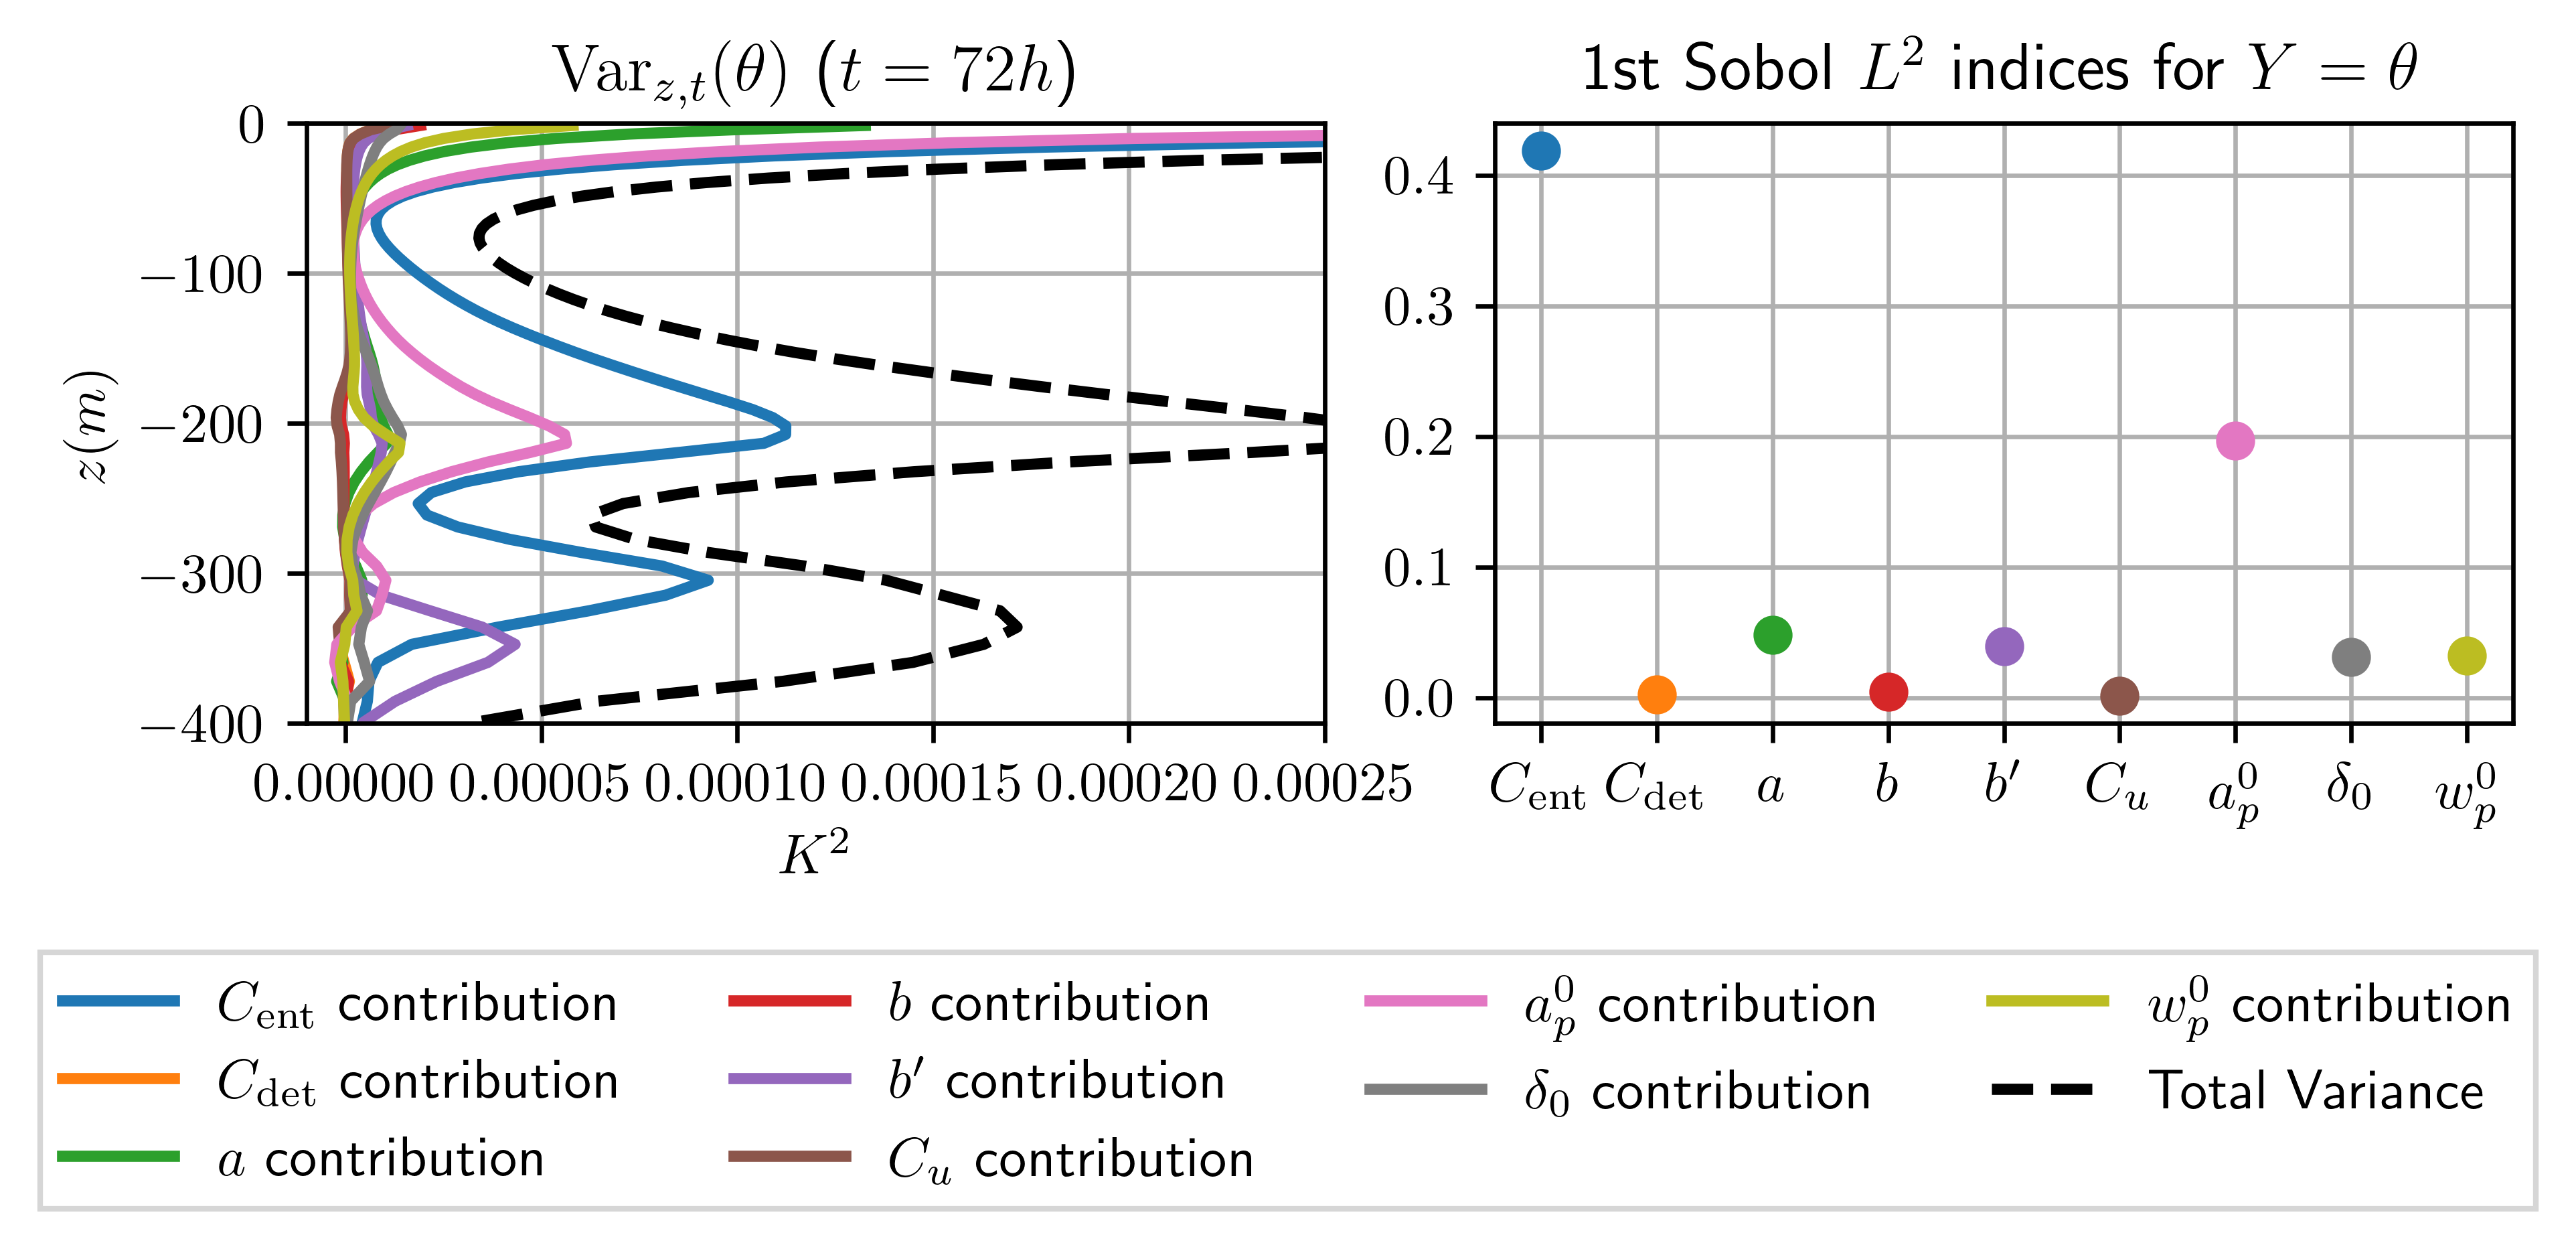
\includegraphics[width=\textwidth]{figures/analysis_of_variance_FC5002048.png}
    \caption{Analysis of temperature variance for the experiment FC500. Left panel: pointwise total variance (black dashed) at $t=\SI{72}{h}$, and individual contributions of input parameters plotted against depth. Right panel: first order Sobol' $L^2$ indices of each input parameter.}
    \label{fig: sobol FC500}
\end{figure}
%
\begin{figure}
    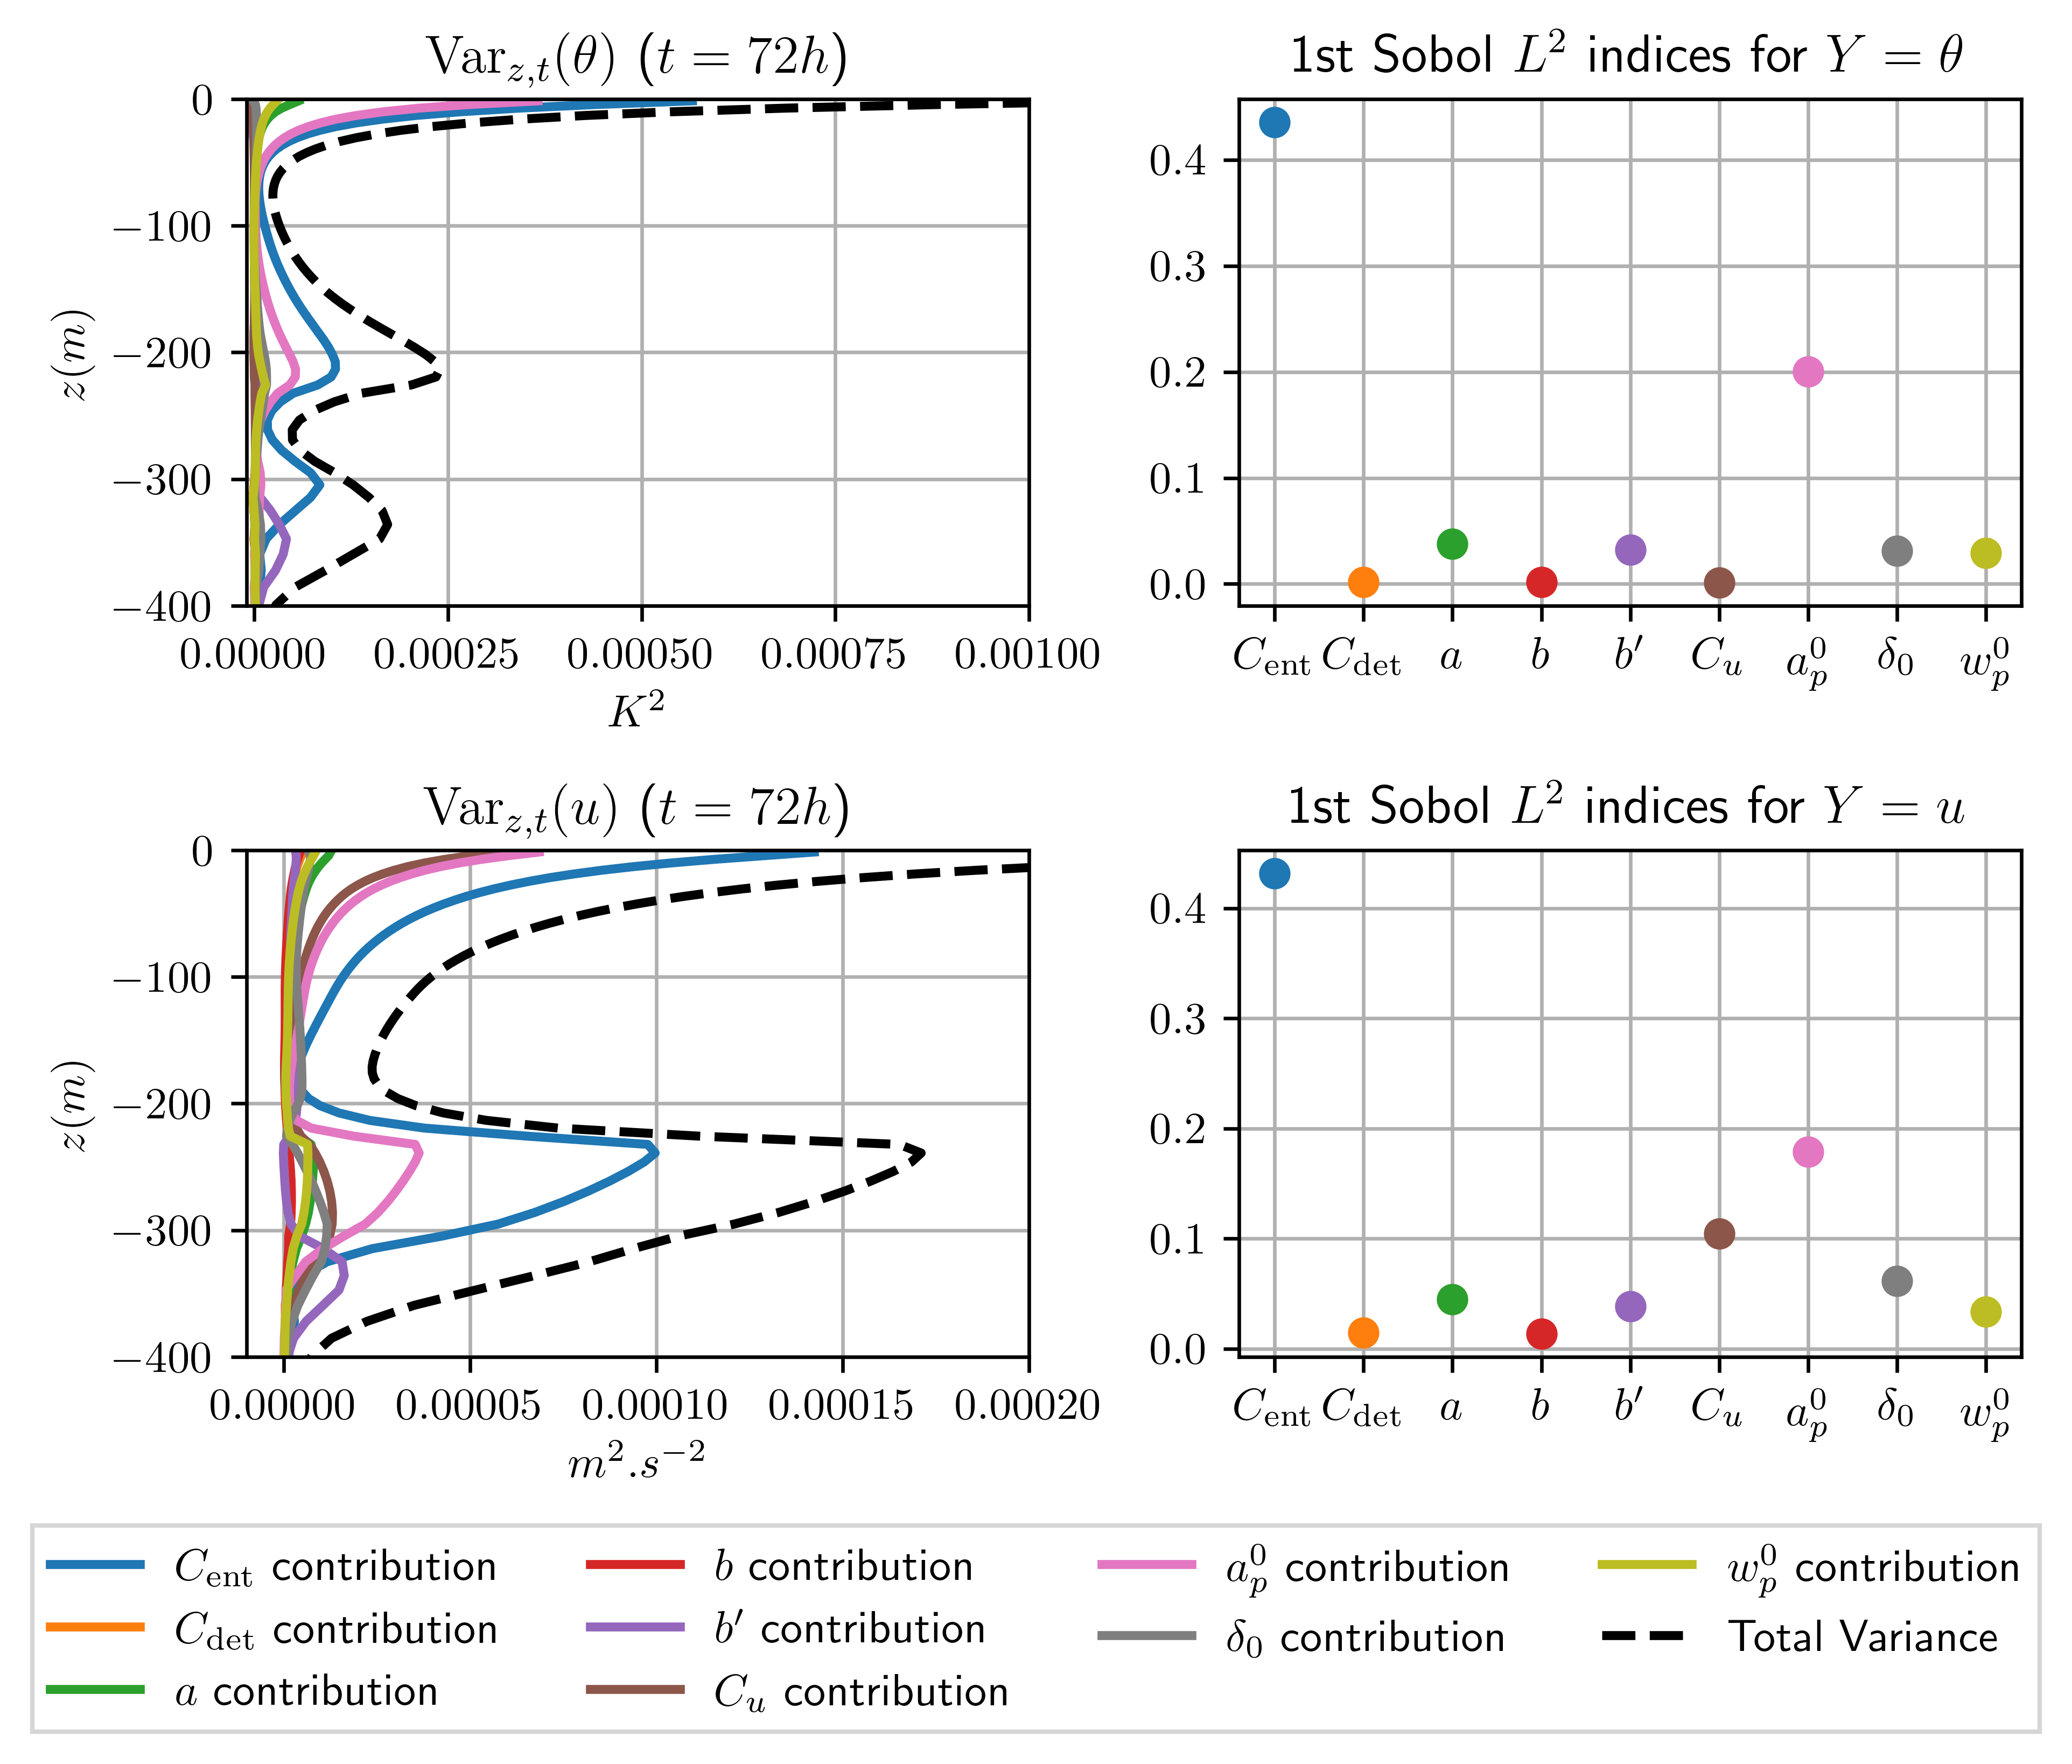
\includegraphics[width=\textwidth]{figures/analysis_of_variance_W005_C500_NO_COR2048.png}
    \caption{Variance analysis for the experiment W005\_C500. Upper panels: analysis of temperature variance. Lower panels: analysis of zonal velocity variance. See fig. \ref{fig: sobol FC500} for details.}
    \label{fig: sobol W005_C500}
\end{figure}
%
\begin{figure}
    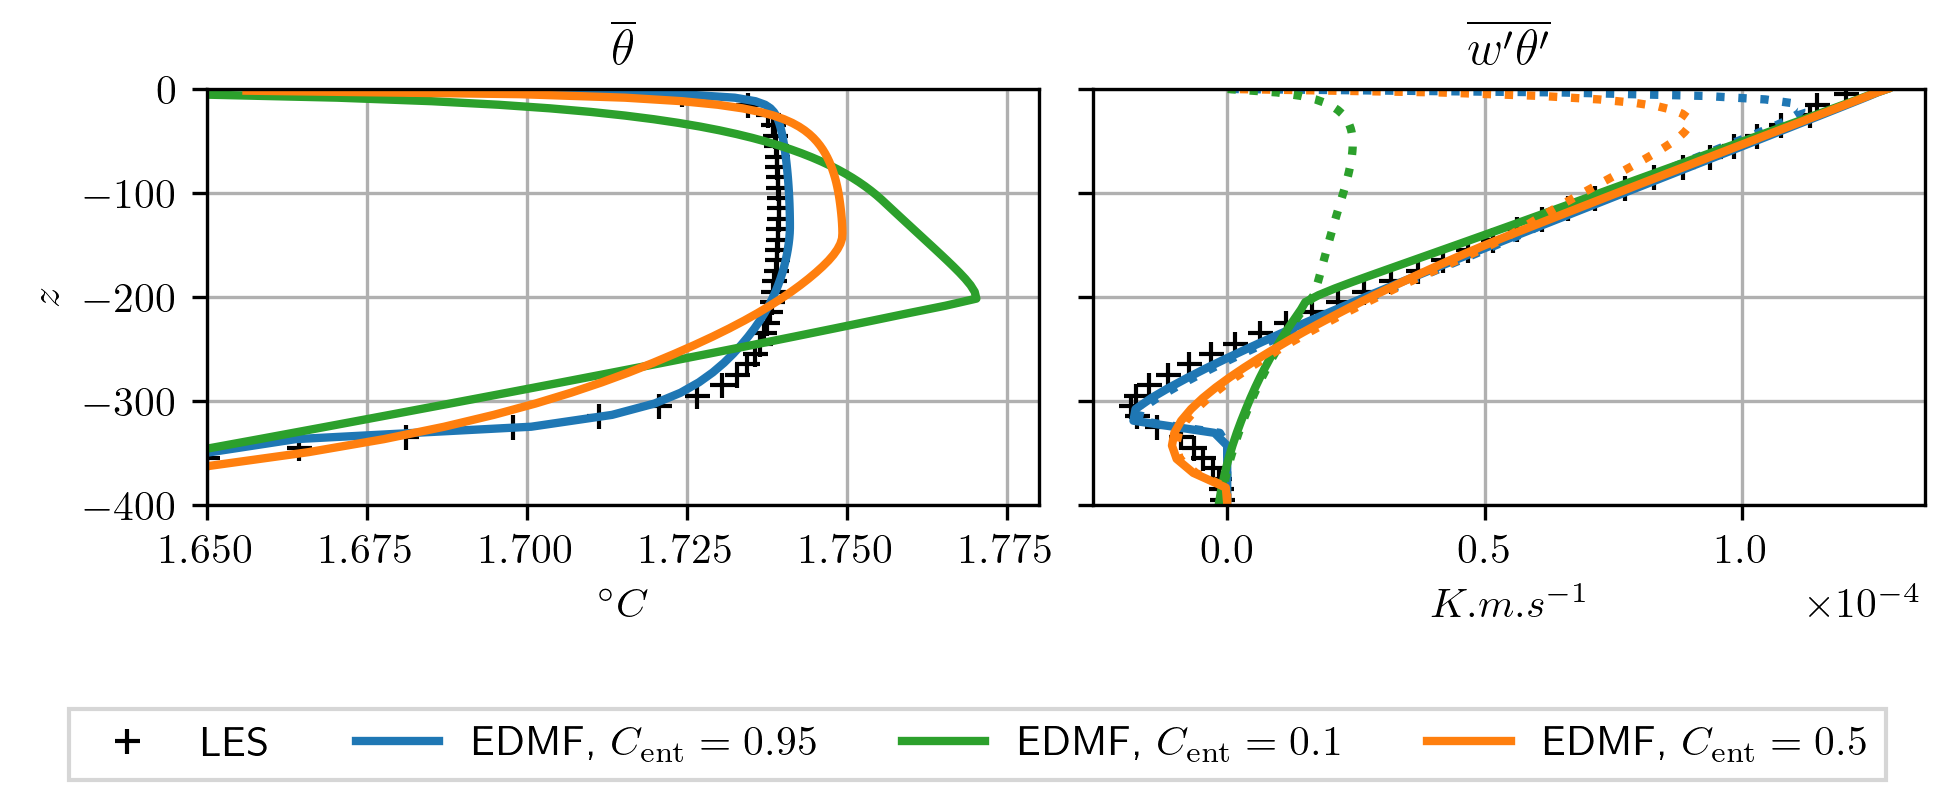
\includegraphics[width=\textwidth]{figures/FC50072h_t_wt.png}
    \caption{Vertical profiles of temperature (left) and temperature fluxes (right) obtained from LES (black dots) and EDMF with varying $C_{\rm ent}$ parameter. Other parameters are kept to nominal values, see chap. \ref{chap: EDMF2}.}
    \label{fig: beta1 FC500}
\end{figure}
%
%
\par As a summary, $C_{\rm ent}$ and $a_p^0$ are the most influential parameters since they control the activation of the MF scheme. In order to have a finer knowledge of the influence of other parameters when the MF is activated, we propose now to fix $C_{\rm ent}$ and $a_p^0$ to their nominal values and perform again the sensitivity analysis. We acknowledge that instead of fixing the two parameters, it could have been more relevant to change the prior uniform distribution into a Gaussian distribution centered on nominal values. Results of the analysis are presented on figure \ref{fig: sobol beta1_ap0_W005_C500} for the case W005\_C500 (similar results for FC500 are not shown). For temperature, $L^2$ Sobol' indices indicates that $b'$ contributes to 40\% of the variance, $w_p^0$ to 20\%, $a$ to 11\% and $\delta_0$ to 9\%. Contributions of other parameters are negligible. For zonal velocity, $L^2$ Sobol' indices indicates that $b'$ contributes to 26\% of the variance, $C_u$ to 24\%, $w_p^0$ to 18\%, $a$ and $\delta_0$ to 13\%.  
%
\par Pointwise variance of both temperature and velocity (left panels of figure \ref{fig: sobol beta1_ap0_W005_C500}) shows maxima at the surface and around $z \simeq \SI{-330}{m}$. The shallow maximum of temperature variance around $z \simeq \SI{-200}{m}$ does not exceed 10\% of the deepest maximum. Thus imposing the activation of MF by fixing $C_{\rm ent}$ and $a_p^0$ greatly reduced the variance attributed to ED-dominated regimes. The surface maximum of variance of temperature is mainly due to $a$ and $w_p^0$ contributions, while for zonal velocity it is mainly due to $C_u$. Regarding the deep maximum, $b'$ is the parameter contributing the most for both temperature and zonal velocity.   
%
%
\begin{figure}
    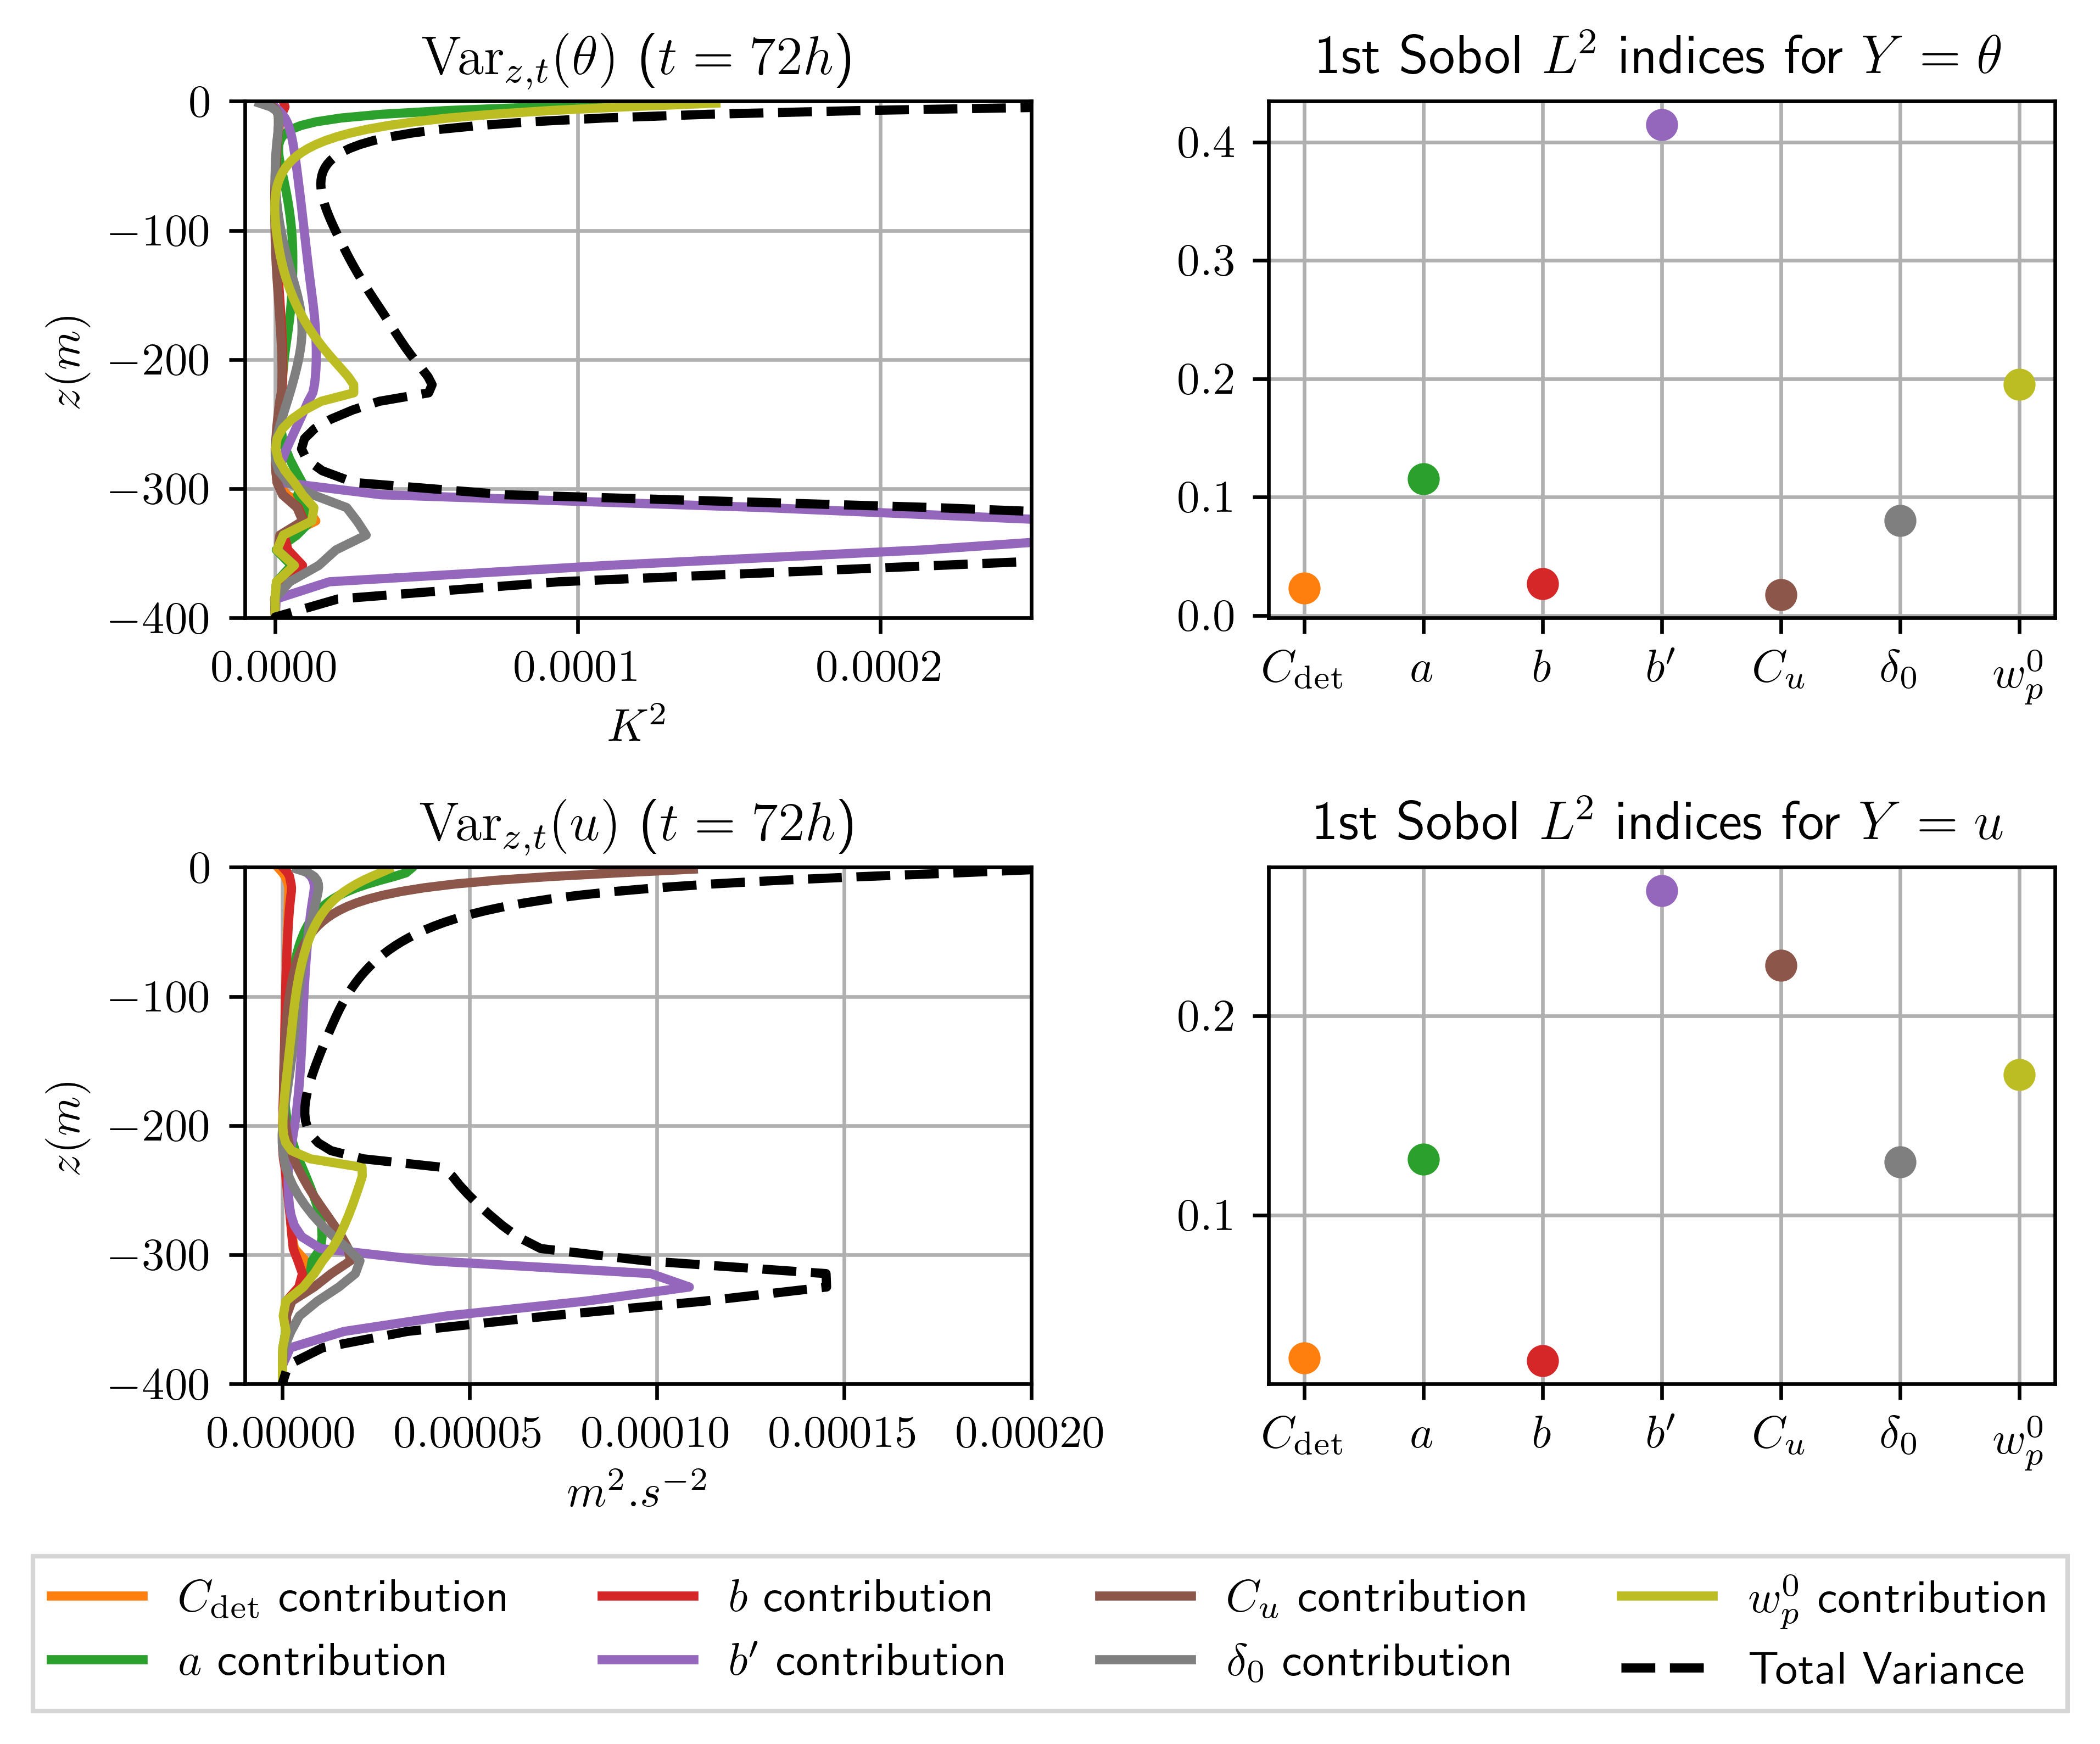
\includegraphics[width=\textwidth]{figures/analysis_of_variance_beta1_ap0_W005_C500_NO_COR2048.png}
    \caption{Same as fig. \ref{fig: sobol W005_C500}, but with fixed parameters $C_{\rm ent}=0.99$ and $a_p^0=0.2$.}
    \label{fig: sobol beta1_ap0_W005_C500}
\end{figure}
%
%%%
%
\par We now turn to inverse uncertainty quantification. 
\section{Parameter estimation}\label{sec: inverse}
%
% \blu{REF inverse problems with neural networks https://arxiv.org/pdf/1808.04730}
Given observations $Y_{\rm obs}$ and a related uncertainty of the measurement $\epsilon_{\rm obs}$, an inverse problem (or parameter estimation) consist in finding appropriate parameters $\bm X$ such that the model output $F(\bm X)$ matches\footnote{Observations and model outputs do not necessarily belong to the same space, and in such case a projection would be required to perform comparison.} the observations up to the \textit{model error} $\epsilon_{\rm model}$ (which could also depend on $\bm X$). Formally it consists in finding solutions $\bm X$ (in a sense to be defined) to the equation\footnote{For simplicity, in this section we omit the experimental hyperparameters $\bm C_{\rm exp}$ that were introduced in \eqref{eq: model}.}
%
\begin{eqnarray}\label{eq: inverse problem}
    Y_{\rm obs} = F(\bm X ) + \epsilon_{\rm obs} + \epsilon_{\rm model}
\end{eqnarray}
%
while minimizing, or at least reducing, the model error. Comparison between model and observations are quantified via a loss function $\mathcal{J}(\bm X, Y_{\rm obs})$. 
%The goal of state estimation is to minimize the loss function and obtain only the optimal parameters \cite{wunsch_discrete_2006}, while Bayesian estimation seeks to characterize the entire joint distribution of parameters.
%
\subsection{Bayesian inference methodology}
%
In the Bayesian formulation of inverse problems, the uncertainty on the parameters $\bm X$ is treated in a probabilistic sense. All the relevant information about $\bm X$, treated as a random variable, is then encoded in its probability density\footnote{In the Bayesian literature, $\pi (\bm x)$ is sometimes referred to as the \textit{probability distribution} of $\bm X$. Although this is a common misuse of language, we will try to restrict the usage of \textit{distribution} to its exact definition, i.e. the map $A\mapsto \mathbb{P}(\bm X \in A)$.} $\pi (\bm x)$. It is defined such that the probability that $\bm X$ belongs to a certain domain $A \subset \mathbb{R}^d$ (with $d$ the number of parameters) is given by
%
\begin{eqnarray*}
    \mathbb{P}(\bm X \in A) = \int_A \pi(\bm x) \, \dd \bm x
\end{eqnarray*}
% This distribution assigns a probability to some choice of parameters to be the true parameters $C$ (parameters minimizing the metrics in our case):
% \begin{align}
%     \pi(\bm C) = \mathcal{P}(C \in \bm C).
% \end{align}
In this setting, estimating the parameters and finding a solution to the inverse problem \eqref{eq: inverse problem} consists in finding $\pi (\bm x)$. 
To do so, it is assumed that some prior knowledge $\pi_{\rm prior}(\bm x)$ is available before performing any inference (i.e. before the observations are used).
%
The prior density is updated using the observation $Y_{\rm obs}$--also treated as a random variable--to obtain a posterior density $\pi_{\text{posterior}}(\bm x | y)$, informed by the observed value $Y_{\rm obs} = y$. In other words, the probability that $\bm X$ belongs to a certain domain $A$, \textit{conditioned} on the observation $Y_{\rm obs} = y$, is now given by
%
\begin{eqnarray*}
    \mathbb{P}(\bm X \in A | Y_{\rm obs} = y) = \int_A \pi_{\text{posterior}}(\bm x | y) \, \dd \bm x
\end{eqnarray*}
%
The density conditioned on the observation can be computed via Bayes formula
%
\begin{eqnarray*}
    \pi_{\rm posterior}(\bm x |y) = \frac{\pi(y|\bm x) \pi_{\rm prior}(\bm x)}{\pi(y)}
\end{eqnarray*}
%
where $\pi(y|\bm x)$, named \textit{likelihood function}, encodes the probability of observing $y$ under different model parameters $\bm x$.
Now assume that model and observations errors are Gaussian, i.e. $\epsilon_{\rm model} \sim \mathcal{N}(0,\sigma_{\rm model}^2), \epsilon_{\rm obs} \sim \mathcal{N}(0,\sigma_{\rm obs}^2)$ where $\sigma_{\rm model}$ and $\sigma_{\rm obs}$ are the respective standard deviations. Then the inverse problem equation \eqref{eq: inverse problem} is equivalent to set that $Y_{\rm obs}$ conditioned on the parameters $\bm X$ is also a Gaussian variable centered on the model output $F(\bm X)$, i.e.
%
\begin{eqnarray*}
    (Y_{\rm obs} | \bm X) \sim \mathcal{N}\parenthese{F(\bm X), \sigma_{\rm obs}^2 + \sigma_{\rm model}^2}
\end{eqnarray*} 
%
Equivalently, the likelihood is given by\footnote{The proportionality symbol $\propto$ is used to indicate that we omit any constant factor that does not depend on $\bm x$.}
%
\begin{eqnarray*}
    \pi(y|\bm x) \propto \exp\parenthese{-\frac{\norm{F(\bm x) - y}^2}{2(\sigma_{\rm obs}^2 + \sigma_{\rm model}^2)}}  
\end{eqnarray*}
%
where the norm $\|\, \cdot \, \|$ is the one that has been used to define standard deviations. The posterior density is then 
%
\begin{eqnarray}\label{eq: posterior}
    \pi_{\text{posterior}}(\bm x | y) \propto \exp\parenthese{-\underbrace{\frac{\norm{F(\bm x) - y}^2}{2(\sigma_{\rm obs}^2 + \sigma_{\rm model}^2)}}_{\mathcal{J}(\bm x,y)}} \pi_{\text{prior}}(\bm x)
\end{eqnarray} 
%
Written this way, there is a clear correspondence between the Bayesian framework and the minimization of a loss function $\mathcal{J}(\bm x, y)$.
%
% For this purpose, a user-defined \textit{likelihood} function $\mathcal{L}$ is used to encode the probability of observations given some parameters. It is typically computed via the loss function $\mathcal{J}(\bm x, y)$ characterizing the difference between model outputs and observations:
% %
% \begin{align*}
%     \mathcal{L}(y | \bm x) \propto \exp(- \mathcal{J}(\bm x,y))
% \end{align*}
% %
% Using Bayes' theorem, the likelihood function is used to derive the posterior distribution:
% \begin{align*}
%     \pi_{\text{posterior}}(\bm x | y) \propto \mathcal{L}(y | \bm x) \pi_{\text{prior}}(\bm x) \propto \exp(- \mathcal{J}(\bm x,y)) \pi_{\text{prior}}(\bm x)
% \end{align*}
%
Moreover, if a certain value $\bm x$ generates a model output "far" from the observation, i.e. $\mathcal{J}(\bm x,y) \gg 1$, then $\bm x$ is unlikely, i.e. $\pi_{\text{posterior}}(\bm x | y) \simeq 0$.
%  Assuming that model and observation errors can be modeled as Gaussian noise with standard deviations $\sigma_{\rm model}$ and $\sigma_{\rm obs}$, a loss function can be defined as 
%
% \begin{eqnarray*}
    % \mathcal{J}(\bm x, y) = \frac{\norm{F(\bm x) - y}^2}{\sigma_{\rm obs}^2 + \sigma_{\rm model}^2 }
% \end{eqnarray*}

% \blu{clarifier que si bruit est gaussien, alors on a rigoureusement que la likelihood c'est une exponentielle!!}
% \\
\par In practice, we use synthetic "observations", i.e. coming from high resolution Large Eddy Simulations (LES). The observation error $\sigma_{\rm obs}$ can be inferred by varying the resolution, spatial domain, discretization scheme and subgrid turbulence parameterizations \cite{couvreux_processbased_2021}. Due to time and computing limitations, we were not able to perform such quantification. Model error is complex to infer a priori, since it is intrinsically based on model knowledge everywhere in the parameter space. In \citeA{couvreux_processbased_2021}, the authors considered $\sigma_{\rm model} $ as a user-defined tolerance to error. Alternatively, \citeA{souza_uncertainty_2020} proposed to dynamically update $\sigma_{\rm model}$ during the exploration of the parameter space every time $\norm{F(\bm x) - y}^2 < \sigma_{\rm model}^2$ while considering $\sigma_{\rm obs} = 0$. We adopted the first approach, with the order of magnitude of the error given by a prior minimization procedure $\sigma_{\rm model}^2 = \min \norm{F(\bm x) - y}^2$.
%
\par Inferring the posterior density requires to compute the likelihood, and thus to evaluate the model on the whole parameter space. This can be computationally expensive, especially when the number of parameters increases. In our case, the parameterization is relatively fast to evaluate and the Fortran/Python interface \cite<via \texttt{F2PY}>{peterson_f2py_2009} alleviate the need for slow writing and reading of NetCDF files at each evaluation. Thus, we use a "brute-force" Markov Chain Monte Carlo (MCMC) method to directly sample the posterior density. For more expensive models, MCMC can be used jointly with emulators of the model (such as Gaussian processes) to reduce overall cost of the estimation \cite<e.g.>{cleary_calibrate_2021,dunbar_calibration_2021}. Alternatively, computational cost can be reduced by iteratively approximating the posterior density via transport maps \cite<e.g.>{zanger_sequential_2024}: this is a way to "emulate" directly the posterior density, instead of emulating the model outputs. 
%
History matching methods \cite{couvreux_processbased_2021}, designed to identify a given level set of the likelihood, also rely on Gaussian processes emulators to accelerate the exploration of the parameter space. 


\subsection{Numerical implementation and results}   
%
Consistently with the section on Sobol analysis \ref{sec: sobol}, the prior is taken as a uniform distribution on the intervals defined in section \ref{sec: prior}. The propagation of this prior uncertainty to outputs of the model was already illustrated on figures \ref{fig: andrew prior FC500} and \ref{fig: andrew prior WC500}, and the specific contribution of each parameter was unveiled via Sobol' analysis. As for Sobol' analysis, we chose a loss function based on $L^2$ norms, 
%
\begin{eqnarray*}
    \mathcal{J} = \frac{\norm{\overline{\theta}-\overline{\theta}_{\rm LES} }^2_{L^2} }{(\sigma^\theta_{\rm obs})^2 + (\sigma^\theta_{\rm model})^2} \frac{1}{2t_0 H}  + \frac{\norm{\overline{\bm u}_h-\overline{\bm u}_{h,{\rm LES} }}^2_{L^2} }{(\sigma^u_{\rm obs})^2 + (\sigma^u_{\rm model})^2} \frac{1}{2t_0 H} 
\end{eqnarray*}
%
where $\norm{(\cdot)}^2_{L^2} = \int_{0}^{t_0} \int_{-H}^{0} (\cdot)^2 \, \dd t \, \dd z $. We use the efficient Differential-Evolution Metropolis(Z) \cite{terbraak_differential_2008} implementation of the MCMC method, provided via the Python library \texttt{PyMC} \cite{abril-pla_pymc_2023}. As recommended for this method, the parameter space is explored by 9 chains consisting of $N=50000$ model evaluations. The quality and convergence of the method is assessed in Appendix \ref{apdx: quality_of_MCMC}.
%
\par To visualize the posterior density conditioned on the LES cases FC500 and WC\_500, we plot on figure \ref{fig: MCMC pairplot} the 2D marginals, e.g.
%
\begin{eqnarray*}
    \pi_{\text{2D marg.}} (x_1,x_2|y) = \int \pi_{\text{posterior}}(x_1,x_2,x_3,\ldots,x_d | y) \, \dd x_3 \ldots \dd x_d
\end{eqnarray*}
%
and the 1D marginals, e.g.,
%
\begin{eqnarray*}
    \pi_{\text{1D marg.}} (x_1|y) = \int \pi_{\text{posterior}}(x_1,x_2\ldots,x_d | y) \, \dd x_2 \ldots \dd x_d
\end{eqnarray*}
%
%
\begin{figure}
    % 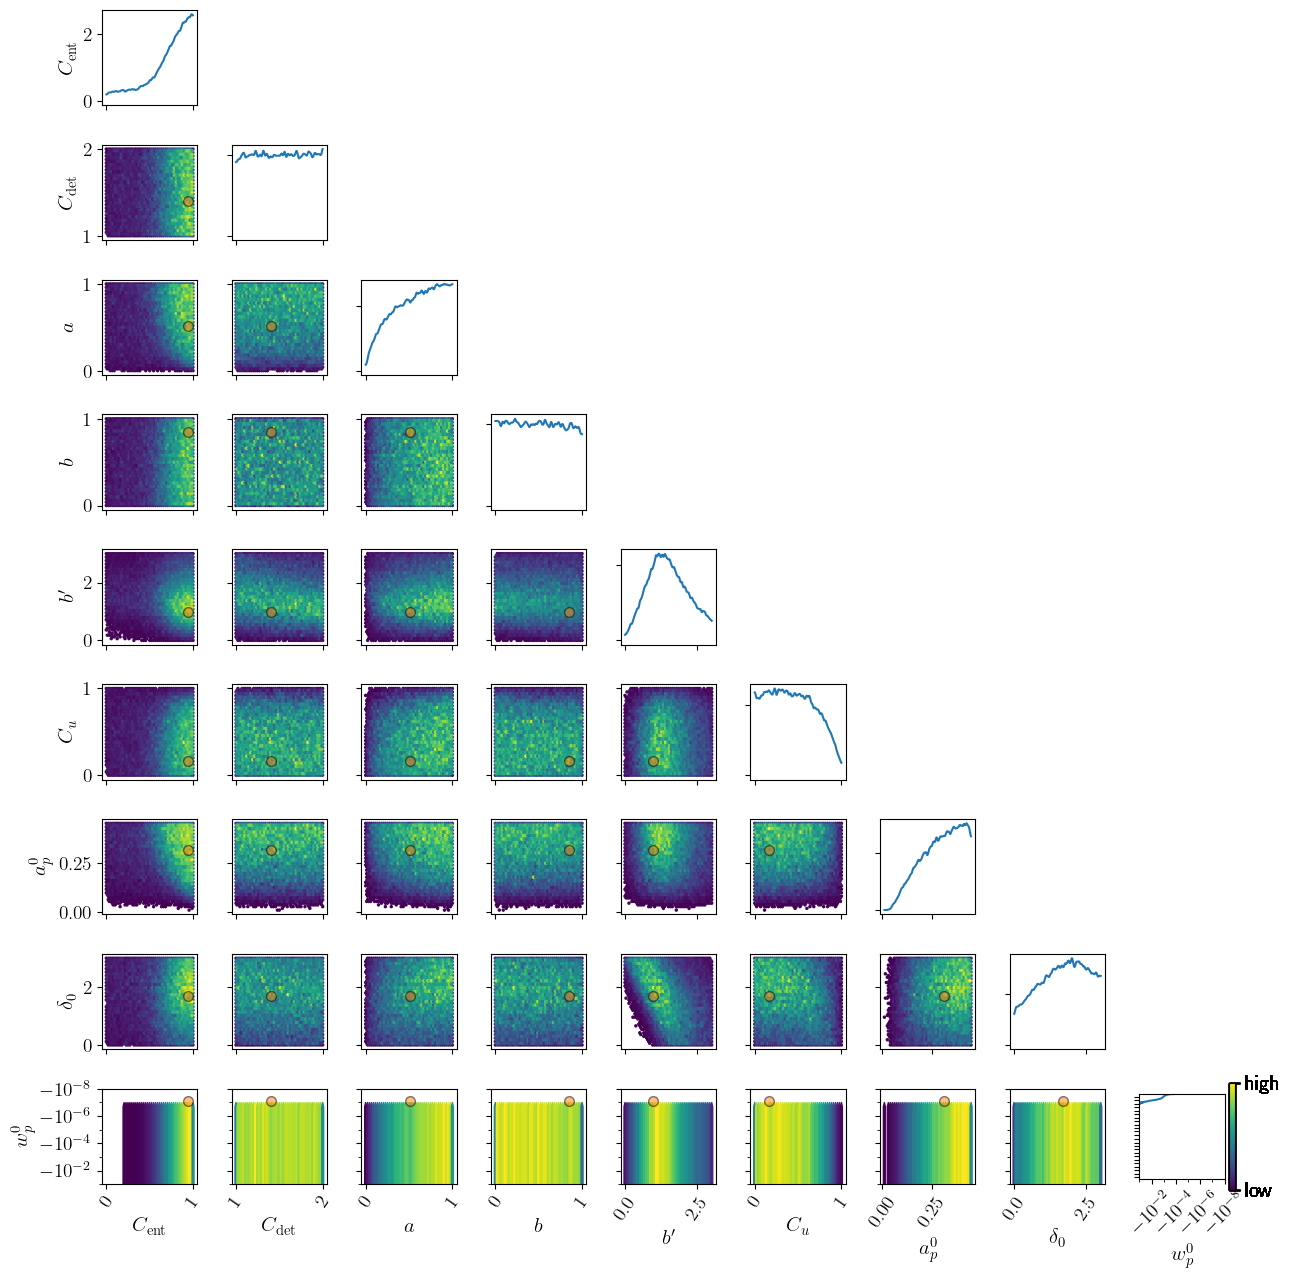
\includegraphics[width=\textwidth]{figures/MCMC_pairplot.pdf}
    \includegraphics[width=\textwidth]{figures/MCMC_pairplot_logwp0.pdf}
    \caption{Estimated 2D and 1D marginals of the posterior density, conditioned on experiments FC500 and W005\_C500. The orange dots represent the maximum a posteriori estimate. Black squares and dotted lines represent the mean value of each parameter. For 1D and 2D marginals, density scales are arbitrary since the posterior density is not normalized, i.e. estimated up to a multiplicative constant.}
    \label{fig: MCMC pairplot}
\end{figure}
%
\par After conditioning on observations, the uncertainty on $C_{\rm ent}$, $b'$ and $w_p^0$ has been greatly reduced, while the uncertainty on $a$, $a_p^0$, $C_u$ and $\delta_0$ has been moderately reduced. The usage of LES data did not allow to reduce the uncertainty on $C_{\rm det}$ and $b$, suggesting that the experiments used are not informative for these parameters, consistent with the insensitivity revealed by Sobol' analysis. 
%
The maximum a posteriori (MAP) estimate $\bm X_{\rm MAP}$, defined as the point of the parameter space that maximizes the posterior density, i.e. $\bm X_{\rm MAP} = \operatorname{argmax}_{\bm x} \pi_{\text{posterior}}(\bm x | y)$ is plotted with orange dots on figure \ref{fig: MCMC pairplot}. It corresponds to the minimum that would give an optimization algorithm on the loss function. 
% Apart for $C_{\rm ent}$, the MAP estimate of $w_p^0$ and other parameters do not lie in regions of high density of the 2D marginals. This suggests that interactions between $C_{\rm ent}$ and $w_p^0$ generate important variability in the likelihood. 
To visualize the propagation of posterior uncertainty to the model outputs, we plot on figures \ref{fig: andrew FC500} and \ref{fig: andrew WC500} an ensemble of 500 model outputs, obtained by sampling from the posterior density. Uncertainties on temperature, zonal velocity and there respective fluxes are greatly reduced, while there still remain large uncertainties on TKE and its transport. Since we used a loss function based on temperature and horizontal velocity, this result indicates that parameters generating realistic temperature and velocity profiles do not necessarily constrain profiles of TKE and TKE flux. However, for these latter outputs, a region of high density is clearly identifiable, indicating some robustness of the parameterization. In the two experiments, ED fluxes (which are directly influenced by TKE) are small compared to MF fluxes, which could explain the lack of constraint on TKE and its flux. 
%
As exposed on fig. \ref{fig: MCMC pairplot}, the posterior density describes parameters that are dependent. Thus, one cannot use Sobol' analysis anymore to attribute the remaining variability of the outputs to specific parameters. Alternatively, Shapley values could have been computed to provide a measure of sensitivity to parameters following the posterior distribution \cite{owen_shapley_2017}.
%
%
\begin{figure}
    \includegraphics[width=\textwidth]{figures/MCMC_FC500_andrew_N500.pdf}
    \caption{An ensemble of model outputs (blue lines) generated by 500 parameters sampled from the \textit{posterior} distribution, for the experiment FC500 at $t=\SI{72}{h}$. The ensemble mean (black continuous line) and standard deviations (black dashed lines) are represented.  }
    \label{fig: andrew FC500}
\end{figure}
%
\begin{figure}
    \includegraphics[width=\textwidth]{figures/MCMC_W005_C500_NO_COR_andrew_N500.pdf}
    \caption{Same as fig. \ref{fig: andrew FC500}, but for the experiment W005\_C500.}
    \label{fig: andrew WC500}
\end{figure}
%
%=======================================================================
% \subsection{History matching}
% %
% \blu{faire petit historique sur HM et dire que là ce qu'on détaille, c'est le HM de Hourdin Couvreux}
% History matching is a methodology for model calibration that focuses on identifying regions of the parameter space that produce acceptable outputs compared to observations, for a given tolerance. The sampling of the parameter space is 
% %
% \subsubsection{Methodology}
% %
% \subsubsection{Interpretation in the Bayesian framework}
% %
% \blu{regarder si c'est pas fait dans papier originels}

% \blu{Ref pour calibration schéma TKE \citeA{vignon_designing_2024}}
%
%=======================================================================
%
\section{Conclusion}
%
%Résumé résultats
In this chapter, we have investigated the forward and inverse propagation of uncertainty in the EDMF parameterization. We first performed a global sensitivity analysis to identify the most influential parameters on the model outputs, regardless of observational data. We found that $C_{\rm ent}$ and $a_p^0$ are the most influential parameters, since they control the activation of the mass-flux scheme. Then, we performed a Bayesian inference to estimate the full posterior density of the parameters using a simple MCMC algorithm, conditioned on synthetic observations obtained from Large Eddy Simulations (LES). 
%Critique 2 obs...
\par The presented work intends to illustrate potentials and limitations of the Bayesian methodology. The main limitation of this study is the lack of observational data, since we used only two different LES experiments. Actually, this criticism could be slightly tempered: since the mixed layer $h$ is evolving in time, the two experiments are dynamically exploring some parts of the experiment's non-dimensional parameter space $(Ri*,h/L_{Ob})$ (see section \ref{sec: turbulent scales}). However, reliable results should obviously be obtained with more observations. Collecting existing datasets \cite{vanroekel_kpp_2018,wagner_formulation_,garanaik_new_2024} in a user-friendly database and building new ones to fully explore this parameter space are goals of the ANR project "Plume", to which this thesis is strongly connected. 
%
\par Using the two experiments, the "brute-force" MCMC algorithm used for Bayesian inference already took $\sim 20$ hours to run on 9 CPU cores. This is a reasonable time for a first exploration of the parameter space but prohibits the use of MCMC as a tool for daily tests of new development features, and motivates the use of emulated approaches. We are currently working on the implementation of different tools: \texttt{htexplo} \cite{couvreux_processbased_2021}, a history matching method designed to provide acceptable ranges of parameters, that relies on Gaussian processes emulators of model outputs; and \texttt{SequentialMeasureTransport.jl} \cite{zanger_sequential_2024}, a method that uses transport maps to iteratively approximate complex and peaky posterior densities.   
%
% \begin{tcolorbox}[title=\textbf{Keypoints}]
%     \begin{itemize}
%         \item Sobol' global sensitivity analysis, a rigorous method relying on variance decomposition, is used to identify the most influential parameters of the EDMF parameterization. 
%         \item Entrainment coefficient and plume fractional area at the surface are the most influential parameters, since they control the activation of the mass-flux scheme
%         \item Bayesian inference, via a simple MCMC algorithm, is used to estimate the full posterior density of the parameters, conditioned on LES data.
%         \item With only two LES experiments, MCMC is found to be computationally expensive, motivating the use of emulators or global approximations of the posterior.
%     \end{itemize}
%   \end{tcolorbox}
% %
\paragraph{Acknowledgment} The estimation part of this work has been conducted in collaboration with Benjamin Zanger (in particular for implementation of MCMC algorithms) and Olivier Zahm (for general discussions on Bayesian estimation).
% \\ 
% \blu{TODO, if time remains:
% If time remains:
% \begin{itemize}
%     \item tableau valeurs ltérature pour a et b
%     \item Remise en contexte history matching dans Bayésien
%     \item  Résulats history matching
%     \item  Résultats Benji transport maps
%     \item  TKE in metric
%     \item  extend prior ranges for Cent, a, wp0 etc
%     \item formulation du problème incluant les paramètres de forçage C\_exp, en lien avec la thèse d'Exaucé? 
%     % \item  attain convergence for Sobol w/ log wp0, and interprete total Sobol indices
% \end{itemize}
% }
%
% \appendixsection
\appendix
%
\section{Sensitivity of Sobol' analysis to number of samples} \label{apdx: sensitivity of sobol}
In order to choose a sufficient number of samples $N$, we estimated Sobol' indices and variances for $N=512,1024,2048,4096$ in the case FC500. Results shown on \ref{fig: sensitivity of sobol} indicates that $N=2048$ is sufficient to reach convergence of the estimators.  
%
\begin{figure}
    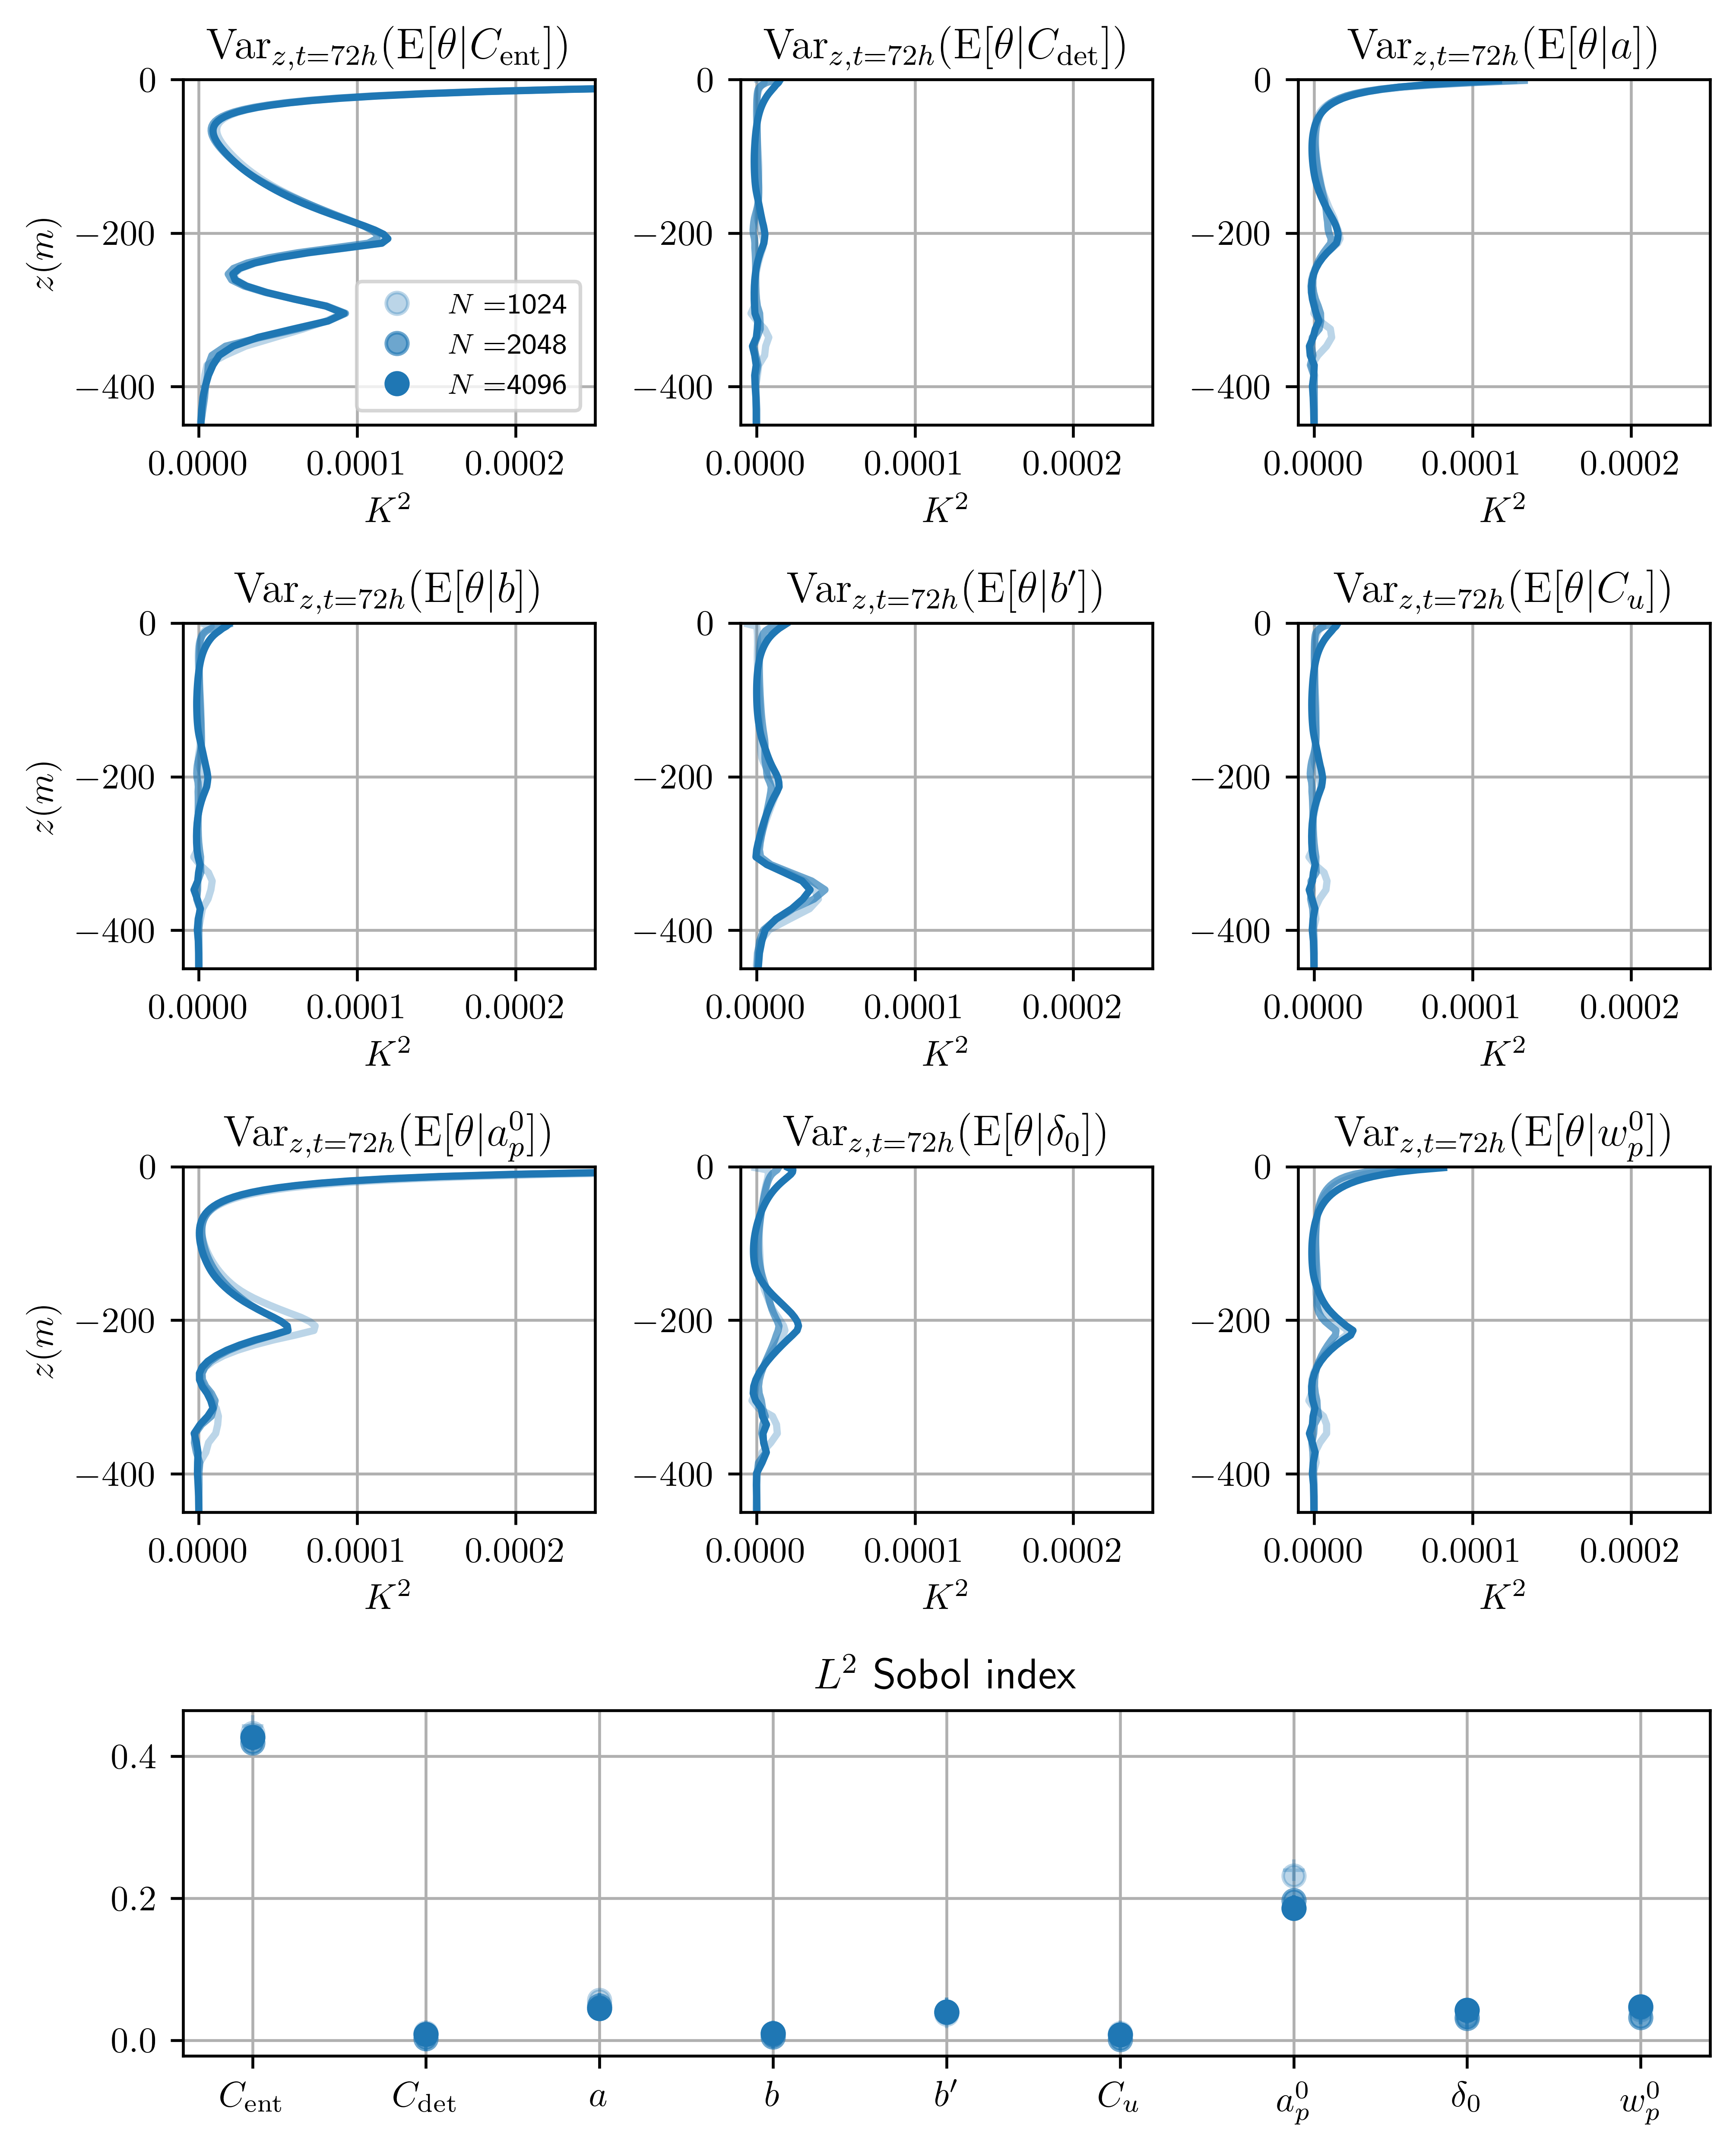
\includegraphics[width=\textwidth]{figures/sensitivity_of_variance_FC500.png}
    \caption{Sensitivity of Sobol' analysis to different samples sizes $N=512,1024,2048,4096$ for the case FC500. Upper panels: pointwise variance contribution of each parameter. Lower panel: first order $L^2$ Sobol' indices.}
    \label{fig: sensitivity of sobol}
\end{figure}
%%
%
%
%
\section{Quality of MCMC}\label{apdx: quality_of_MCMC}
%
There are multiple qualitative and quantitative methods to evaluate the quality of MCMC results.
First, visually, we compare the \emph{mixing of different chains}.
To do so, we plot the sample density of different chains and see if they agree for all parameters (fig. \ref{fig:mixing_of_MCMC_chains}).
\begin{figure}
	\centering
	\includegraphics[width=\textwidth]{figures/MCMC_mixing.pdf}
	\caption{Mixing of the different MCMC chains. The 1D marginal densities for each parameter (left panels) agrees for all chains. On the right panels, values of each parameter for the 9 chains are presented.}\label{fig:mixing_of_MCMC_chains}
\end{figure}
If the densities of the different chains would not agree well, this is an indicator that MCMC had not yet converged, and more samples would have been needed.
%
\par Next, we look at more quantitative methods.
A widely used one is $\hat{R}$, which compares the variance in a chain with the variance between all chains.
Let $W_k$ be the variance and $E_k$ the expectation in the $k$-th chain.
Define the average chain variance $W$ and the between chains variance $B$ as
\begin{align}
	W &= \frac{1}{m} \sum_{k=1}^{m} W_{k} \\
	B &= \frac{1}{m-1} \sum_{k=1}^{m} \left(E_k - \frac{1}{m} \sum_{k=1}^{m} E_k\right)
\end{align}
and define
\begin{equation}
	\hat{R} = \sqrt{\frac{n-1}{n} + \frac{B}{W}}.
\end{equation}
Note that for $n \rightarrow \infty$, $B \rightarrow 0$, while this is not the case for $W$. Hence, a converged MCMC chain has a value close to $1$.

Finally, let us talk about the \emph{effective sample size (ESS)}.
This quantitative indicator has its origin in importance sampling, and loosely speaking, tells you how many samples the given MCMC samples would correspond to independent samples from the target distribution.
The estimation of a linear estimator using the MCMC samples for the target distribution, converges approximately with $\sigma^2 / \mathrm{ESS}$. 
ESS and $\hat{R}$ are plotted on figure \ref{fig:forest_of_MCMC_chains}.
%
\begin{figure}
	\centering
	\includegraphics[width=\textwidth]{figures/MCMC_forest.pdf}
	\caption{Mixing of the different MCMC chains. The 1D marginal densities for each parameter (left panels) agrees for all chains. On the right panels, values of each parameter for the 9 chains are presented.}\label{fig:forest_of_MCMC_chains}
\end{figure}
%%
%% ------------------------------------------------------------------------ %%
%% Open Research statement 
%% ------------------------------------------------------------------------ %%
\section*{Open Research}
%%
\subsection*{Data Availability Statement}
Data from the Lion mooring (located in the Gulf of Lion; Mediterranean sea) are 
freely accessible from \citeA{bosse_lion_2023}. The output from LES simulations 
and the initial and surface boundary conditions for the Hymex/ASICS-MED experiments
are available at the Zenodo archive https://zenodo.org/records/10619442.
%%
\subsection*{Software Availability Statement}
The LES model Méso-NH can be downloaded at http://mesonh.aero.obs-mip.fr/mesonh57. All the SCM codes used in this study have been made available and can be found 
at the Zenodo archive https://zenodo.org/records/10619442. It includes the single-column model with Eddy-Diffusivity 
Mass-Flux turbulent closure developed from scratch. The latter consists of low-level code written in Fortran 
interfaced with Python using F2PY \cite{peterson_f2py_2009}. The single-column simulations analyzed in
this study can be executed from a high-level Python driver code without any intervention 
on the Fortran code. The high-level Python driver code and scripts to reproduce the figures 
are available in the Zenodo archive. The Fortran code contains inline documentation following 
the FORD (Fortran Documenter) format. 
%
%% ------------------------------------------------------------------------ %%
%% Acknowledgments
%% ------------------------------------------------------------------------ %%
\acknowledgments
The authors would like to thank Hilary Weller and two anonymous reviewers for their constructive comments to help improve our manuscript. 
This work was supported by the \textit{institut des Mathématiques pour la Planète Terre} (iMPT) through 
the project ``Coherent sub-grid scale modeling for ocean climate models''.
This study was carried out as part of the technological defense project  PROTEVS2 under the 
auspices of the French Ministry of the Armies / DGA, was funded in part by l’Agence Nationale de la Recherche (ANR), project
ANR-23-CE01-0009. MP was supported by a PhD fellowship from Ecole Normale Supérieure Paris.
The authors are extremely grateful to Jean-Luc Redelsperger for his essential contributions to 
the MESO-NH model. 
   
%% ------------------------------------------------------------------------ %%
%% References and Citations
\bibliography{references}
\end{document}



More Information and Advice:

%% ------------------------------------------------------------------------ %%
%
%  SECTION HEADS
%
%% ------------------------------------------------------------------------ %%

% Capitalize the first letter of each word (except for
% prepositions, conjunctions, and articles that are
% three or fewer letters).

% AGU follows standard outline style; therefore, there cannot be a section 1 without
% a section 2, or a section 2.3.1 without a section 2.3.2.
% Please make sure your section numbers are balanced.
% ---------------
% Level 1 head
%
% Use the \section{} command to identify level 1 heads;
% type the appropriate head wording between the curly
% brackets, as shown below.
%
%An example:
%\section{Level 1 Head: Introduction}
%
% ---------------
% Level 2 head
%
% Use the \subsection{} command to identify level 2 heads.
%An example:
%\subsection{Level 2 Head}
%
% ---------------
% Level 3 head
%
% Use the \subsubsection{} command to identify level 3 heads
%An example:
%\subsubsection{Level 3 Head}
%
%---------------
% Level 4 head
%
% Use the \subsubsubsection{} command to identify level 3 heads
% An example:
%\subsubsubsection{Level 4 Head} An example.
%
%% ------------------------------------------------------------------------ %%
%
%  IN-TEXT LISTS
%
%% ------------------------------------------------------------------------ %%
%
% Do not use bulleted lists; enumerated lists are okay.
% \begin{enumerate}
% \item
% \item
% \item
% \end{enumerate}
%
%% ------------------------------------------------------------------------ %%
%
%  EQUATIONS
%
%% ------------------------------------------------------------------------ %%

% Single-line equations are centered.
% Equation arrays will appear left-aligned.

Math coded inside display math mode \[ ...\]
 will not be numbered, e.g.,:
 \[ x^2=y^2 + z^2\]

 Math coded inside \begin{equation} and \end{equation} will
 be automatically numbered, e.g.,:
 \begin{equation}
 x^2=y^2 + z^2
 \end{equation}


% To create multiline equations, use the
% \begin{eqnarray} and \end{eqnarray} environment
% as demonstrated below.
\begin{eqnarray}
  x_{1} & = & (x - x_{0}) \cos \Theta \nonumber \\
        && + (y - y_{0}) \sin \Theta  \nonumber \\
  y_{1} & = & -(x - x_{0}) \sin \Theta \nonumber \\
        && + (y - y_{0}) \cos \Theta.
\end{eqnarray}

%If you don't want an equation number, use the star form:
%\begin{eqnarray*}...\end{eqnarray*}

% Break each line at a sign of operation
% (+, -, etc.) if possible, with the sign of operation
% on the new line.

% Indent second and subsequent lines to align with
% the first character following the equal sign on the
% first line.

% Use an \hspace{} command to insert horizontal space
% into your equation if necessary. Place an appropriate
% unit of measure between the curly braces, e.g.
% \hspace{1in}; you may have to experiment to achieve
% the correct amount of space.


%% ------------------------------------------------------------------------ %%
%
%  EQUATION NUMBERING: COUNTER
%
%% ------------------------------------------------------------------------ %%

% You may change equation numbering by resetting
% the equation counter or by explicitly numbering
% an equation.

% To explicitly number an equation, type \eqnum{}
% (with the desired number between the brackets)
% after the \begin{equation} or \begin{eqnarray}
% command.  The \eqnum{} command will affect only
% the equation it appears with; LaTeX will number
% any equations appearing later in the manuscript
% according to the equation counter.
%

% If you have a multiline equation that needs only
% one equation number, use a \nonumber command in
% front of the double backslashes (\\) as shown in
% the multiline equation above.

% If you are using line numbers, remember to surround
% equations with \begin{linenomath*}...\end{linenomath*}

%  To add line numbers to lines in equations:
%  \begin{linenomath*}
%  \begin{equation}
%  \end{equation}
%  \end{linenomath*}



